%%%%%%%%%%%%%%%%%%%%%%%%%%%%%%%%%%%%%%%%%%%%%%%%
\input{preamble.ltx}

% correct bad hyphenation here; separate each word by a space
\hyphenation{op-tical net-works semi-conduc-tor}

%%%%%%%%%%%%%%%%%%%%%%%%%%%%%%%%%%%%%%%%%%%%%%%%
\begin{document}

\title{Discrete-Time Signals} % titles are generally capitalized except for words such as a, an, and, as, at, but, by, for, in, nor, of, on, or, the, to, and up, which are usually not capitalized unless they are the first or last word of the title. Linebreaks \\ can be used within to get better formatting as desired. Do not put math or special symbols in the title.

\author{
	{\small
	%\renewcommand{\arraystretch}{1.3}
	\begin{tabular}{l l l}
    & \multicolumn{2}{c}{\tiny \textcolor[rgb]{0.9,0.9,0.9}{Participated in \& did the coursework [Y/N]?}} 
    \\ 
		DELA~CRUZ,~Juan~A.~(10312345) & Y & 
\includegraphics[height=5ex]{JAD_signature}
		\\ 
		FRANCO,~Nat~B.~(10354321)     & Y & 
\includegraphics[height=5ex]{NBF_signature}
		\\ 
		RIANZARES,~Max~C.~(10314325)  & N & 
\includegraphics[height=5ex]{MCR_signature}
		\\ 		
	\end{tabular}
	}
% for author names; note positions of commas and nonbreaking spaces ( ~ ) LaTeX will not break a structure at a ~ so this keeps an author's name from being broken across two lines.
\thanks{\CrmD\protect\\} %<--Do not delete this \thanks{\CrmD\protect\\} 
 \thanks{Coursework Starting Date: \hspace{1ex} Apr. 19, 2005}
\thanks{Submission Date: \hspace{1ex} Apr. 26, 2005}} 

\markboth{\makebox[\columnwidth]{Coursework \# 01 \hfill}%
\hspace{\columnsep}\makebox[\columnwidth]{\hfill}}%
{} % header

\IEEEpubid{\makebox[\columnwidth]{COURSE CODE - SECTION \hfill DLSU}%
\hspace{\columnsep}\makebox[\columnwidth]{ \hfill {\tiny\textcolor[rgb]{0.4,0.4,0.4}{\prsDy}}}} % footer

\maketitle % for making the title area






\section{Abstract}
The summary text goes here. Limit to 150 words. The summary text is a single paragraph summarizing the report's significant aspects. Do not cite references in the summary.


\section{Conspectus}
\label{sec:cnspcts}

\IEEEpubidadjcol % needed in the second column of the first page if using \IEEEpubid

\subsection{What are the objectives of the coursework?}

\begin{enumerate}
\item To \ldots;
\item To \ldots;
\end{enumerate}	
	
\subsection{How does the coursework fit the course and previously done coursework?}
By:
\begin{enumerate}
\item Up to two lines per item.
\item Up to two lines per item.
\end{enumerate}	


	
\subsection{How were the objectives achieved?}
By:
\begin{enumerate}
\item Up to two lines per item.
\item Up to two lines per item.
\end{enumerate}
	
\subsection{What are the key results and generalizations?}
The key results are:
\begin{enumerate}
\item Up to two lines per item.
\item Up to two lines per item.
\end{enumerate}

 








\section{Principles}
\label{sec:concps}

\subsection{What are the necessary and relevant concepts, principles, theoretical and design considerations for understanding the coursework and for supporting the correct results?}
\label{sec:nrcp}
\begin{enumerate}
\item Up to two lines per item.
\item Up to two lines per item.
\end{enumerate}

\subsection{How does any new component, not covered in previous coursework, function?}
\label{sec:nfxn}
By:
\begin{enumerate}
\item Up to two lines per item.
\item Up to two lines per item.
\end{enumerate}
	
\subsection{What figures, equations, and/or tables could support your answers in Sec.~\ref{sec:nrcp} and Sec.~\ref{sec:nfxn}?}
\begin{enumerate}
\item Up to two lines per item. Figure \ldots shows \ldots
\item Up to two lines per item. Table \ldots shows \ldots
\end{enumerate}
	
\subsection{Did you cite more than two publications in your answers in Sec.~\ref{sec:nrcp} and Sec.~\ref{sec:nfxn}?}
Yes.
	
\subsection{Did you cite any online source in your answers in Sec.~\ref{sec:nrcp} and Sec.~\ref{sec:nfxn}?}
No.
  
	
	
	
	
	
	
	
	
	


\section{Methodology}

\subsection{How does your implementation in Sec.~\ref{sec:implem} achieve the objectives?}
By:
\begin{enumerate}
\item Up to two lines per item.
\item Up to two lines per item.
\end{enumerate}
	
\subsection{Why does your implementation in Sec.~\ref{sec:implem} achieve the objectives?}
Because:
\begin{enumerate}
\item Up to two lines per item.
\item Up to two lines per item.
\end{enumerate}
	
\subsection{How does your evaluation in Sec.~\ref{sec:eval} achieve the objectives?}
By:
\begin{enumerate}
\item Up to two lines per item.
\item Up to two lines per item.
\end{enumerate}
	
\subsection{Why does your evaluation in Sec.~\ref{sec:eval}  achieve the objectives?}
Because:
\begin{enumerate}
\item Up to two lines per item.
\item Up to two lines per item.
\end{enumerate}



\subsection{Implementation}
\label{sec:implem}

Rule of thumb: Implementation is how you made your work; (keywords: implemented, created, made, soldered, programmed, etc.).


\subsubsection{What were the materials used?}
If the presentation would be better and necessary, tabulate your answers here instead of enumeration.
\begin{enumerate}
\item Up to two lines per item.
\item Up to two lines per item.
\end{enumerate}


\subsubsection{What is the summary of the processes used to make the coursework?}
If you wrote a program or made a simulation, you must add statements on how the program or simulation functions in this section.	A pseudocode as shown in Table~\ref{tab:calcxn} is a good example.
\begin{enumerate}
\item Up to two lines per item.
\item Up to two lines per item.
\end{enumerate}

\begin{table}[!b]
	\caption{Pseudocode for the calculation of $y = x^n$}
	\label{tab:calcxn}	
	\centering
	{\footnotesize
	\begin{tabular}{lll}
	\hline
	\hline
	{\bfseries Input(s):} & & \\
	$n$ & : & $n$th power; $n \in \mathbb{Z}^{+}$ \\
	$x$ & : & base value; $x \in \mathbb{R}^{+}$ \\
	\hline
	{\bfseries Output(s):} & & \\
	$y$ & : & result; $y \in \mathbb{R}^{+}$  \\
	\hline
	\hline
	\\
	\end{tabular}
	}
	\begin{algorithmic}[1]
	{\footnotesize
		\REQUIRE $n \geq 0 \vee x \neq 0$
		\ENSURE $y = x^n$
		\STATE $y \Leftarrow 1$
		\IF{$n < 0$}
				\STATE $X \Leftarrow 1 / x$
				\STATE $N \Leftarrow -n$
		\ELSE
				\STATE $X \Leftarrow x$
				\STATE $N \Leftarrow n$
		\ENDIF
		\WHILE{$N \neq 0$}
				\IF{$N$ is even}
						\STATE $X \Leftarrow X \times X$
						\STATE $N \Leftarrow N / 2$
				\ELSE[$N$ is odd]
						\STATE $y \Leftarrow y \times X$
						\STATE $N \Leftarrow N - 1$
				\ENDIF
		\ENDWHILE
	}
	\end{algorithmic}
\end{table}







\subsection{Evaluation}
\label{sec:eval}

Rule of thumb: Evaluation is how you tested your work for correctness; (keywords: measured, tested, compared, simulated, etc.).

\subsubsection{What were your procedures for evaluating the correct outcome of your coursework?}
\begin{enumerate}
\item Up to two lines per item.
\item Up to two lines per item.
\end{enumerate}
	
\subsubsection{What quantities were gathered and how have you obtained them for testing the veracity of your results?}
\begin{enumerate}
\item Up to two lines per item.
\item Up to two lines per item.
\end{enumerate}




















\section{Results and Discussions}

\subsection{How do the results achieve the objectives?}
By:
\begin{enumerate}
\item Up to two lines per item.
\item Up to two lines per item.
\end{enumerate}
	
\subsection{Why do the results achieve the objectives?}
Because:
\begin{enumerate}
\item Up to two lines per item.
\item Up to two lines per item.
\end{enumerate}

\subsection{Are all your results correct in accordance with what you described in Sec.~\ref{sec:eval} evaluation process? Why?} 
Yes/no, because:
\begin{enumerate}
\item Up to two lines per item.
\item Up to two lines per item.
\end{enumerate}
	
\subsection{What is result $X$ (briefly describe it here), what does it mean if it is correct, and how does it contribute to reaching the objectives?}
\label{sec:resn}
		
		\begin{enumerate}		
		\item Refer to the appropriate caption number of your result, i.e. Fig.~$X$ for figure $X$, Table~$X$ for table $X$, etc.	
		\item Interpret result $X$ and the reasons why it was obtained. 
		
		\item Point out and explain apparent discrepancies from principles/concepts/theory if your result is incorrect.
		
		\begin{enumerate}
			\item Explanation 1
			
			\item Explanation 2
		\end{enumerate}
		
		\item Cite existing publication for comparison of your result.
		
		\item Do not present your result as ``It worked'' without an appropriate explanation as such action does not show thorough understanding.
	
						
		\item Repeat Sec.~\ref{sec:resn} for each major result $X$ (i.e. $X$=1, $X$=2, etc.).		
	\end{enumerate}

For example, result $X = 1$ (on the accuracy performance of the enhanced bi-directive method):

\begin{enumerate}
\item Figure \ldots shows that the performance of the system is satisfactory up to 90\%.
\item The result in Figure \ldots was obtained because of the bi-directive mechanism of the proposed architecture.
\item The remaining 10\% accuracy loss is due to the failure of the bi-directive mechanism to \ldots and supported by \ldots.
\item Reference~\cite{Einstein1905} also achieved similar range of results from 85\% to 93\%.
\item \ldots
\end{enumerate}
	
\subsection{Did you cite more than two publications in your answers above (yes/no)?}
Yes.	



















\section{Conclusions}
\label{sec:conc}

\subsection{What are the main points that should be known, remembered, and learned about the coursework?}
\begin{enumerate}
\item Up to two lines per item.
\item Up to two lines per item.
\end{enumerate}

\subsection{What are the gists of the inferences drawn from your results?}

\subsection{Briefly, what are your comments on (1)~your results, and  (2)~future coursework if any?}
\begin{enumerate}
\item Up to two lines per item.
\item Up to two lines per item.
\end{enumerate}	



\section{CRediT Author Statement}

On what contributions to specify, see the terms at \url{www.elsevier.com/researcher/author/policies-and-guidelines/credit-author-statement}.  An example is as follows.  Follow the enumeration below in your report.

\begin{enumerate}
	\item DELA CRUZ, Juan A.: Conceptualization, Methodology, Software, Supervision.
	
	\item FRANCO, Nat B.: Data curation, Writing - Original draft preparation, Validation.
	
	\item RIANZARES, Max C.: Visualization, Investigation. Software, Writing - Reviewing and Editing.
\end{enumerate}



\bibliographystyle{IEEEtran}
\bibliography{references} % references section










\section{Answers to Questions}
\label{sec:ans2ques}

Put your answers to the review/test question(s) of the coursework if included.  Retain the question(s). 

\subsection{Question 1}  
\begin{enumerate}
\item Up to two lines per item.
\item Up to two lines per item.
\end{enumerate}	
	
\subsection{Question 2}  
\begin{enumerate}
\item Up to two lines per item.
\item Up to two lines per item.
\end{enumerate}
	
\subsection{Question 3}  
\begin{enumerate}
\item Up to two lines per item.
\item Up to two lines per item.
\end{enumerate}	







\newpage
\begin{figure*}[!t]
	
\includegraphics[width=\textwidth]{not_a_rubric.pdf} % change rubric.pdf with the specified rubric
\end{figure*}
\cleardoublepage























\appendices

\section{Instructions for Addressing Specific Items in Sec.~\ref{sec:cnspcts} to Sec.~\ref{sec:ans2ques}}

\begin{enumerate}

	\item Do not remove the questions in each section.
	
	\item Generally, use normal font formatting for your answer(s).

	\item Make sure that you cite references that you use. 
		
	\begin{enumerate}
		\item  Most references should be books and not online sources. 
		
		\item \emph{Citing Wikipedia is not allowed}, because the veracity of its contents and authorship can be doubtful.
	\end{enumerate}
	
\end{enumerate}





\section{Usage of This Template}

\begin{enumerate}
	\item The instructions in this template give you guidelines for preparing your report.

	\item Use this document as a template, but format specific items accordingly.
	
	\item When using the files that came with this template, it is suggested that the files and folders are intact, and not located in separate locations.  
	
	\item Graphics/images are stored primarily in the ``figure'' folder. 
	
	\item The rubric for assessment does not count towards the maximum number of pages of your report.
\end{enumerate}




\section{About the Template}

\begin{enumerate}
	\item This template was made with \LaTeX, which is a high-quality typesetting system. 
		
	\begin{enumerate}
		\item \LaTeX\ includes features designed for the production of technical and scientific documentation. 
	
		\item \LaTeX\ is the \textit{de facto} standard for the communication and publication of scientific documents. 
		
		\item \LaTeX\ is available as free software. 
	\end{enumerate}
			
	\item In these appendices are examples of using various \LaTeX\ markup tagging conventions for formatting (headings, figures, tables, equations, etc.), styling, citing, cross-referencing, etc.
		
	\begin{enumerate}
		\item  \emph{\rdfnt{So the reader/user is expected to pay close attention to the examples and features, and adopt and use them accordingly}}. 
		
		\item Please refer to both the original \url{report_format_template.tex} and \url{_README.pdf} files. 
		
		\begin{enumerate}
			\item \rdfnt{Open the the original report\_format\_template.tex} to see how the contents of output file (\url{_README.pdf} or original \url{report_format_template.pdf}) were \LaTeX\ coded.
			
			\item \rdfnt{Open the output file (\url{_README.pdf} or original \url{report_format_template.pdf}) file} to see how the specific \LaTeX\ codes in the original \url{report_format_template.tex} file were generated.
		\end{enumerate}
						
		\item Text in this \textcolor[rgb]{1,1,0}{font color} are blind texts throughout this template to show how a ``printed'' text will look like in such locations.
	\end{enumerate}
	
	\item In using this template, the user is expected to have a working knowledge of \LaTeX, of which~\cite{Oetiker2014} is a good introduction (its latest version can be accessed at \url{http://www.ctan.org/tex-archive/info/lshort}). 
	
	\item This template is adopted and based on IEEE Article Templates and Instructions (~\url{http://www.ieee.org/publications_standards/publications/authors/author_templates.html})~\cite{Shell2015, IEEEMSW2013}--all rights reserved.
\end{enumerate}
		








 

















\section{Example of a Section Heading}
Section text here. 

\subsection{Example of a Subsection Heading}
Subsection text here. 

\subsubsection{Example of a Subsubsection Heading}
Subsubsection text here. 





\section{Referring to Specific Items}

\subsection{Referring to Entries in the Bibliography/References by Citing}

\begin{enumerate}
	\item Citing publications in your document using this template is accomplished using BibTeX.
	
	\item BibTeX is reference management software for formatting lists of references and is used in the LaTeX document preparation system.

	\begin{enumerate}
		\item JabRef is suggested for managing the BibTeX file called \url{references.bib} and other bibliographies. 
		
		\item \url{http://www.mcgill.ca/library/files/library/jabref_guide_2016.pdf} may be a quick guide to using JabRef.
	\end{enumerate}
	
	\item Finding the BibTeX citation on the Web can be one way of filling up necessary bibliography details. 
	
	\item The bibliography format follows the IEEE referencing style, i.e. its corresponding \LaTeX\ code is \verb|\bibliographystyle{IEEEtr}| and the specific BibTeX file is \url{references. bib} and coded as \verb|\bibliography{references}|, noting the extension filename ``.bib'' is omitted.
		
\end{enumerate}

With the BibTeX file \url{references.bib} placed, here is an example of a citation for ISO~80000-2 standard:~\cite{ISO800002}, where \verb|\cite{ISO800002}| is used in which \verb|ISO800002| is the BibTeX~key that is specified in the BibTeX file \url{references.bib}.  Another citation example:~\cite{Einstein1905, Tanenbaum2002}, which is a use of more than one BibTeX~key as a comma-separated list of the argument of \verb|\cite{ }|. Please check the \LaTeX\ code how this argument was accomplished.



	
\subsection{Referring to Sections, Figures, Tables, Equations}	

\begin{enumerate}
	\item In \LaTeX, the specific item (section, figure, table, equation) number is referred to by making a \verb|\label{name}|, wherein \verb|name| is the label name beside the item.

	\item To obtain the item number, refer to it using \verb|\ref{name}| for sections, figures, or tables and using  \verb|\eqref{eqn:name}| for equations; see corresponding examples in this template. 
	
		\item  When referencing your figures and tables within your report, use the abbreviation ``Fig.'' except at the beginning of a sentence: ``Figure~ 2 indicates \ldots .'' 
	
	\item Do not abbreviate ``Table.'' 
	
	\item Refer to ``(1),'' not ``Eq. (1)'' or ``equation (1),'' except at the beginning of a sentence: ``Equation~(1) is ... .''
	
	\item Do not use ``Ref.'' or ``reference'' except at the beginning of a sentence: ``Reference [3] shows ... .'' 
		
	\item If you are quoting specific items of a programming code or command use monospace fonts, e.g. \verb|printf("hello, world\n");|, which is accomplished by using the command \verb|{\ttfamily printf("hello, world\n");}| in \LaTeX. 
	
\end{enumerate}









\section{Examples of Figure and Table Placements}


This template typically puts floats (the term for movable items such as figures and tables) only at the top, even when this results in a large percentage of a column being occupied by floats.



\subsection{Figure in a Single-Column}

Fig.~\ref{fig:mag_v_field} is an example of a single-column floating figure.


\begin{figure}[!tb]
	\centering
	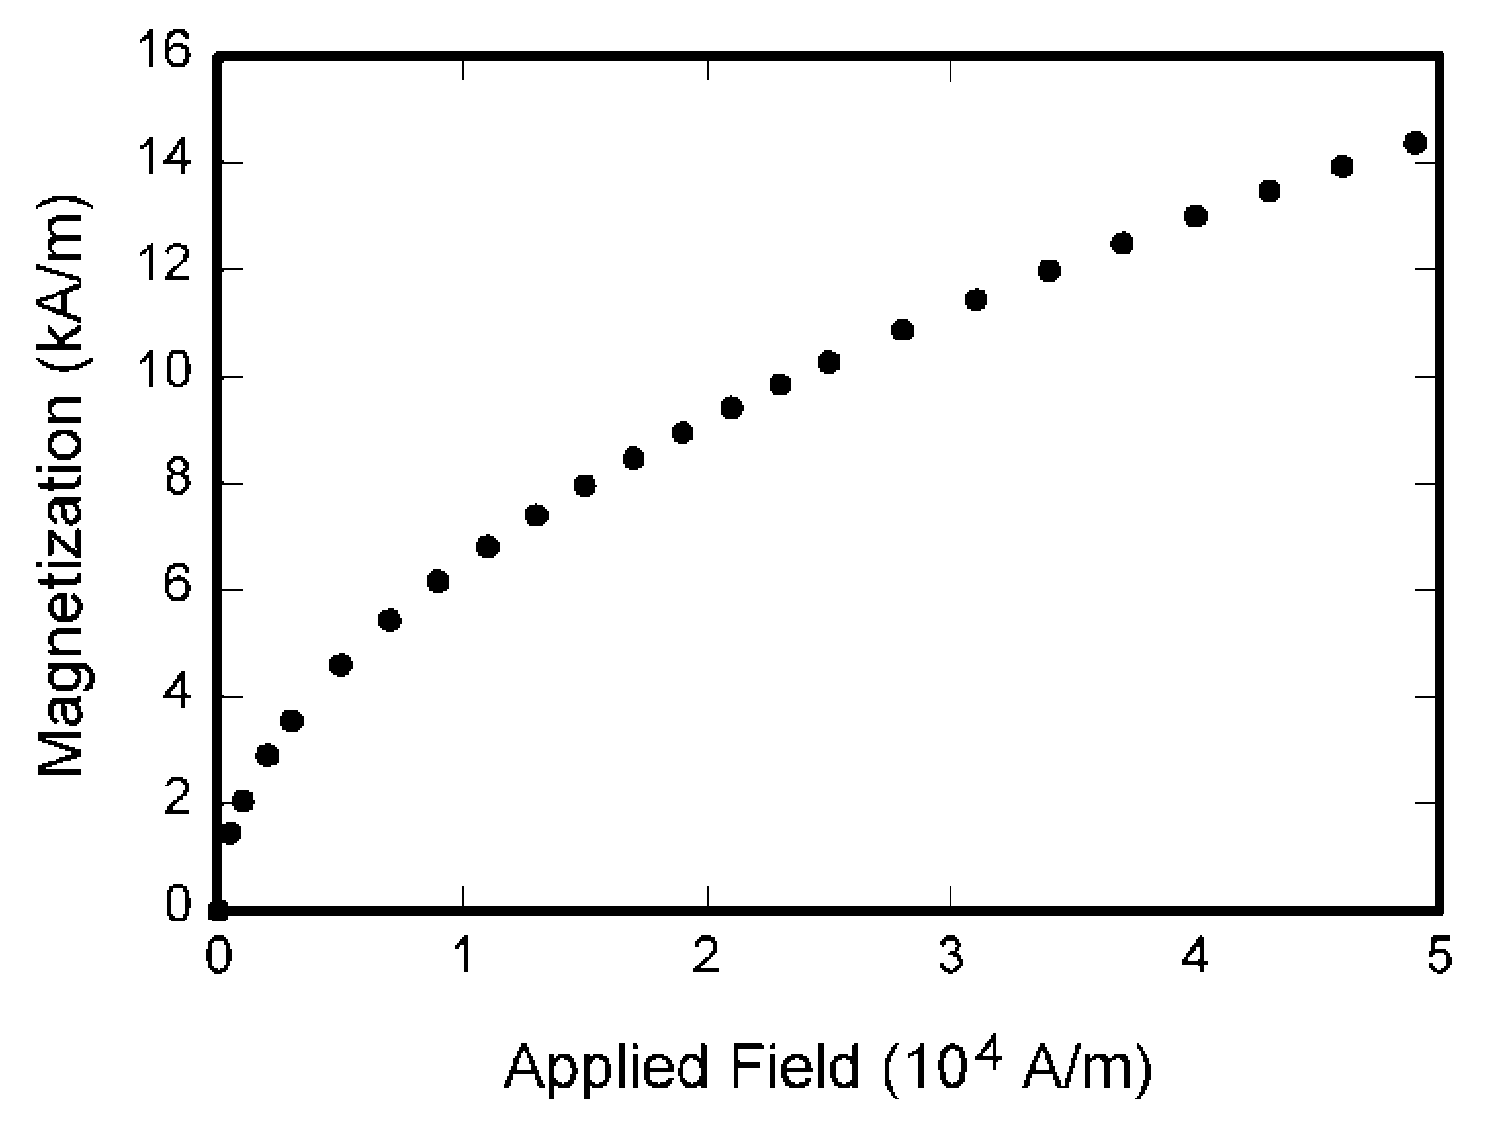
\includegraphics[width=1.0\columnwidth]{Magnetization_vs_Applied_Field}
	\caption{Magnetization as a function of an applied field. In the text body, note that ``Fig.'' is abbreviated and is used for referring to figures. \emph{It is good practice to explain the significance of the figure in the caption.} This is a single-column figure example. PDF/JPG/PNG graphics files are supported under pdf\LaTeX}
	\label{fig:mag_v_field}
\end{figure}





\subsection{Figure/s in Two-Columns}

\begin{enumerate}
	\item In Fig.~\ref{fig:1row_by_2col}, the subfigure \verb|\label| commands are set within each subfloat command, and the \verb|\label| for the overall figure must come after \verb|\caption|. \verb|\hfil| is used as a horizontal separator to get equal spacing. 
	
	\item Watch out that the combined width of all the subfigures on a line does not exceed the text or line width, otherwise a line break will occur.
	
 \item Be aware that for the subfig package to generate the (a), (b), etc., subfigure labels, the optional argument to \verb|\subfloat| must be present. 

	\item Examples:

	\begin{enumerate}
		\item Here is an example of referencing Fig.~\ref{fig:1row_by_2col}. Fig.~\ref{fig:1row_by_2col:mag_v_field1} is the first figure in Fig.~\ref{fig:1row_by_2col} whereas Fig.~\ref{fig:1row_by_2col:mag_v_field2} is the second one.
		
		\item Fig.~\ref{fig:onefigtwocol} is an example of one figure occupying two columns. 
		
		\item Fig.~\ref{fig:2row_by_2col} is an example of four figures occupying two columns.
		
		\item Fig.~\ref{fig:1row_by_4col} is an example of four figures occupying one row.
		
		\item Fig.~\ref{fig:4row_by_1col} is an example of four figures occupying one column
				
	\end{enumerate}
	
	\item If a subcaption is not desired, just leave its contents blank, e.g., \verb|\subfloat[]|.

\end{enumerate}


\begin{figure*}[!tb]
	\centering
	\subfloat[Label of subfigure 1.]{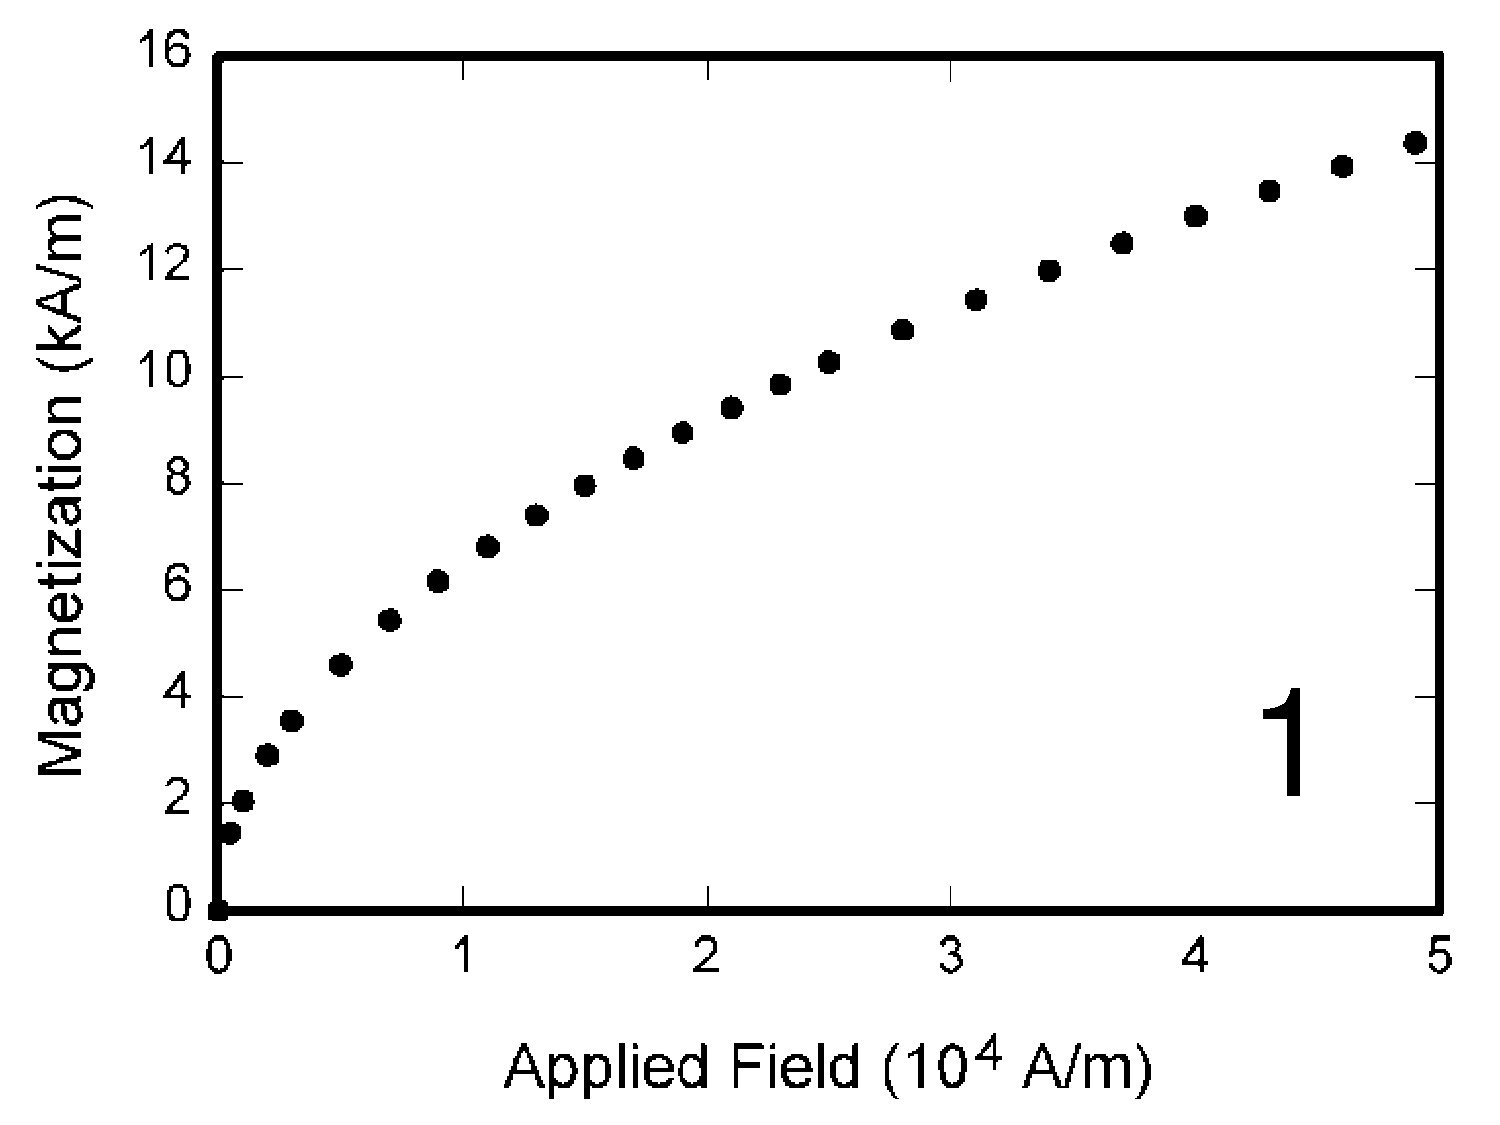
\includegraphics[width=0.9\columnwidth]{Magnetization_vs_Applied_Field_1}%
	\label{fig:1row_by_2col:mag_v_field1}}
	\hfil
	\subfloat[Label of subfigure 2.]{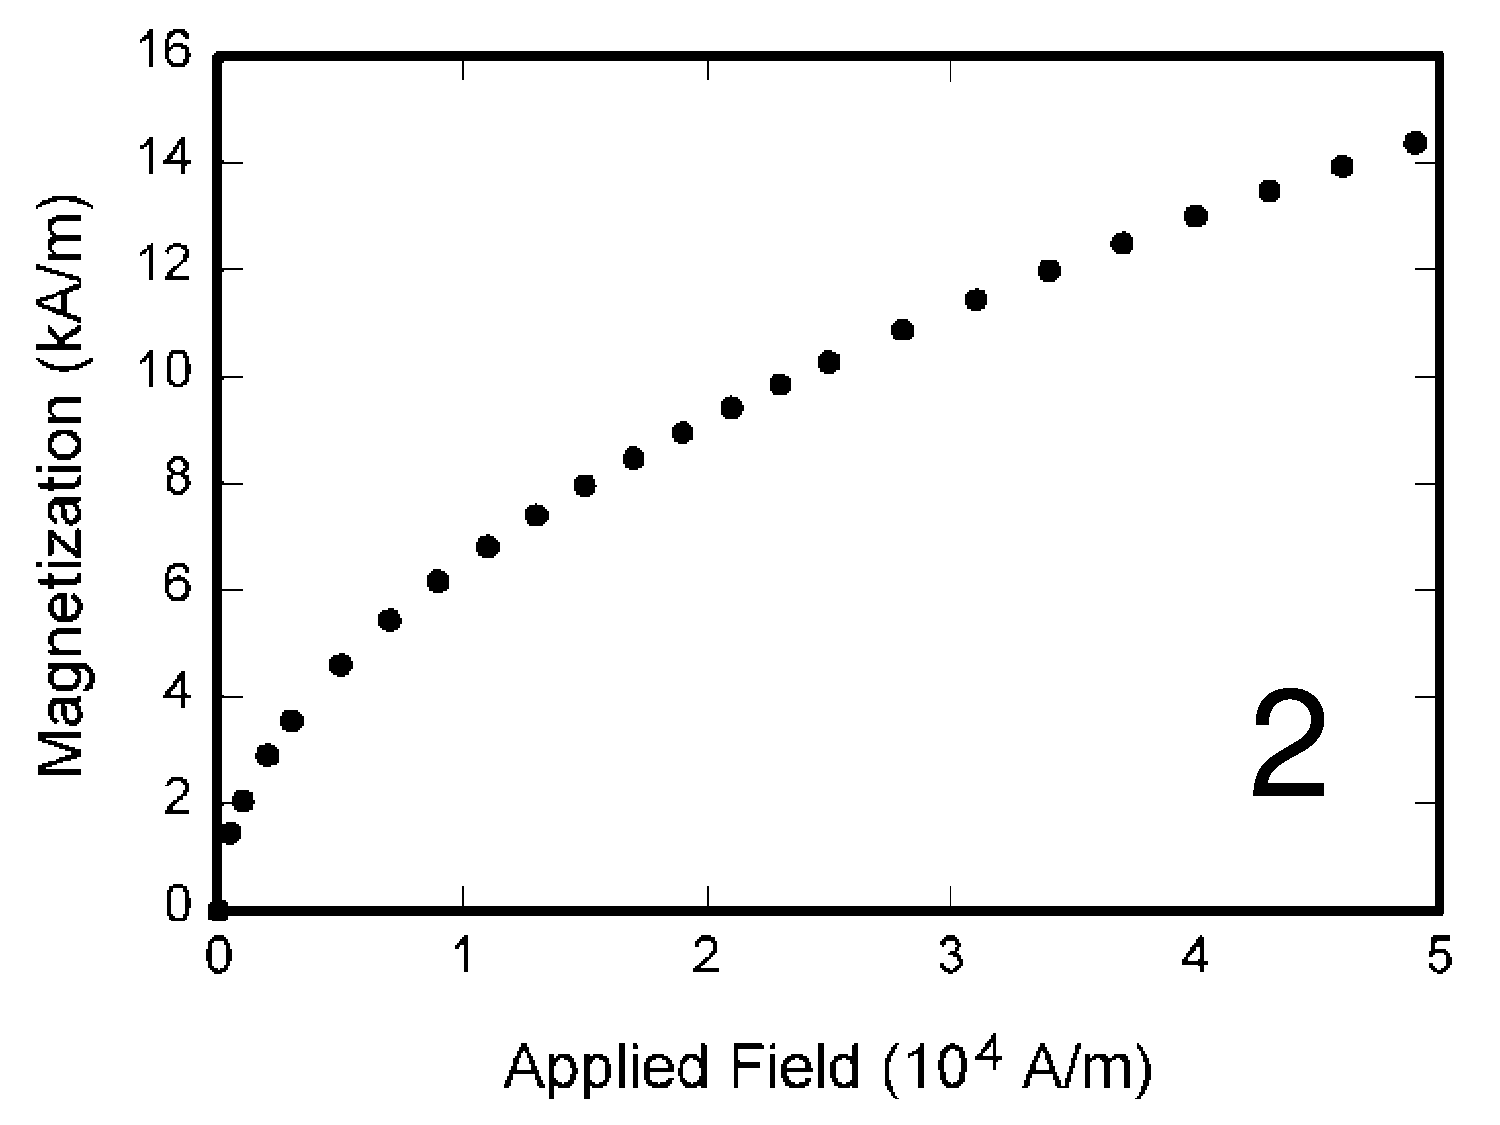
\includegraphics[width=0.9\columnwidth]{Magnetization_vs_Applied_Field_2}%
	\label{fig:1row_by_2col:mag_v_field2}}
	\caption{Example of two figures in two columns.}
	\label{fig:1row_by_2col}
\end{figure*}


\begin{figure*}[!tb]
	\centering
	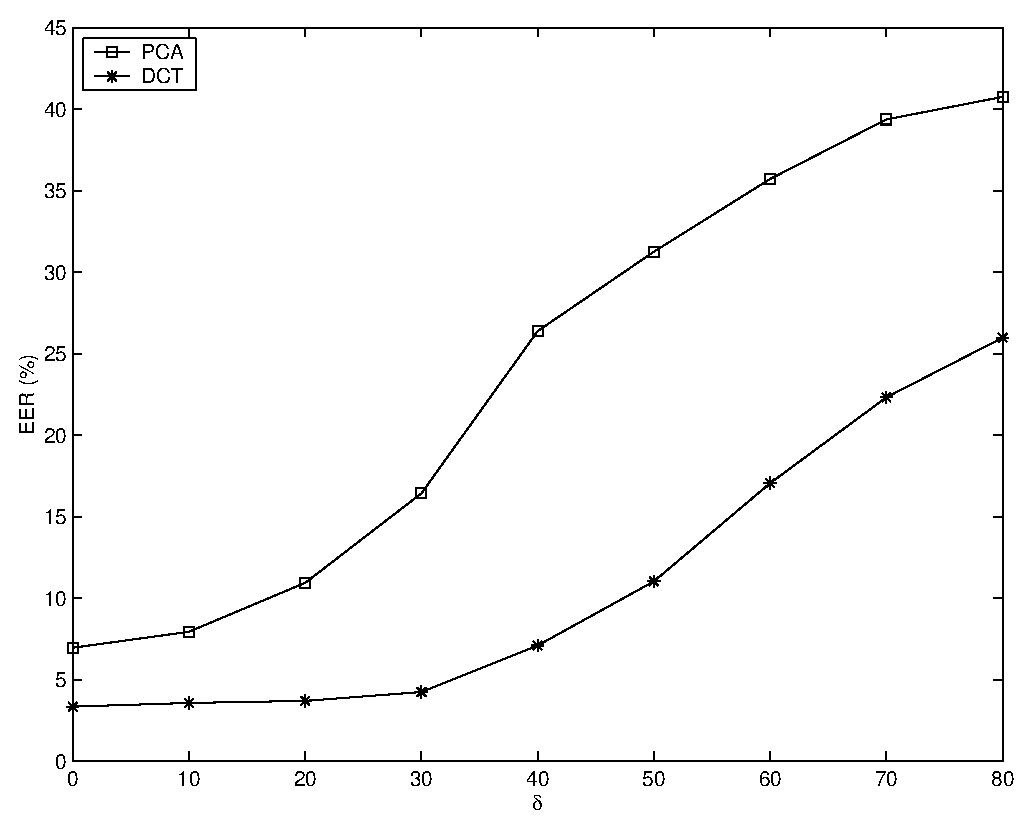
\includegraphics[width=1.8\columnwidth]{Misclassification_Rate}
	\caption{Example of a one figure occupying two columns.}
	\label{fig:onefigtwocol}
\end{figure*}



\begin{figure*}[!tb]
	\centering
	\subfloat[Label of subfigure 1.]{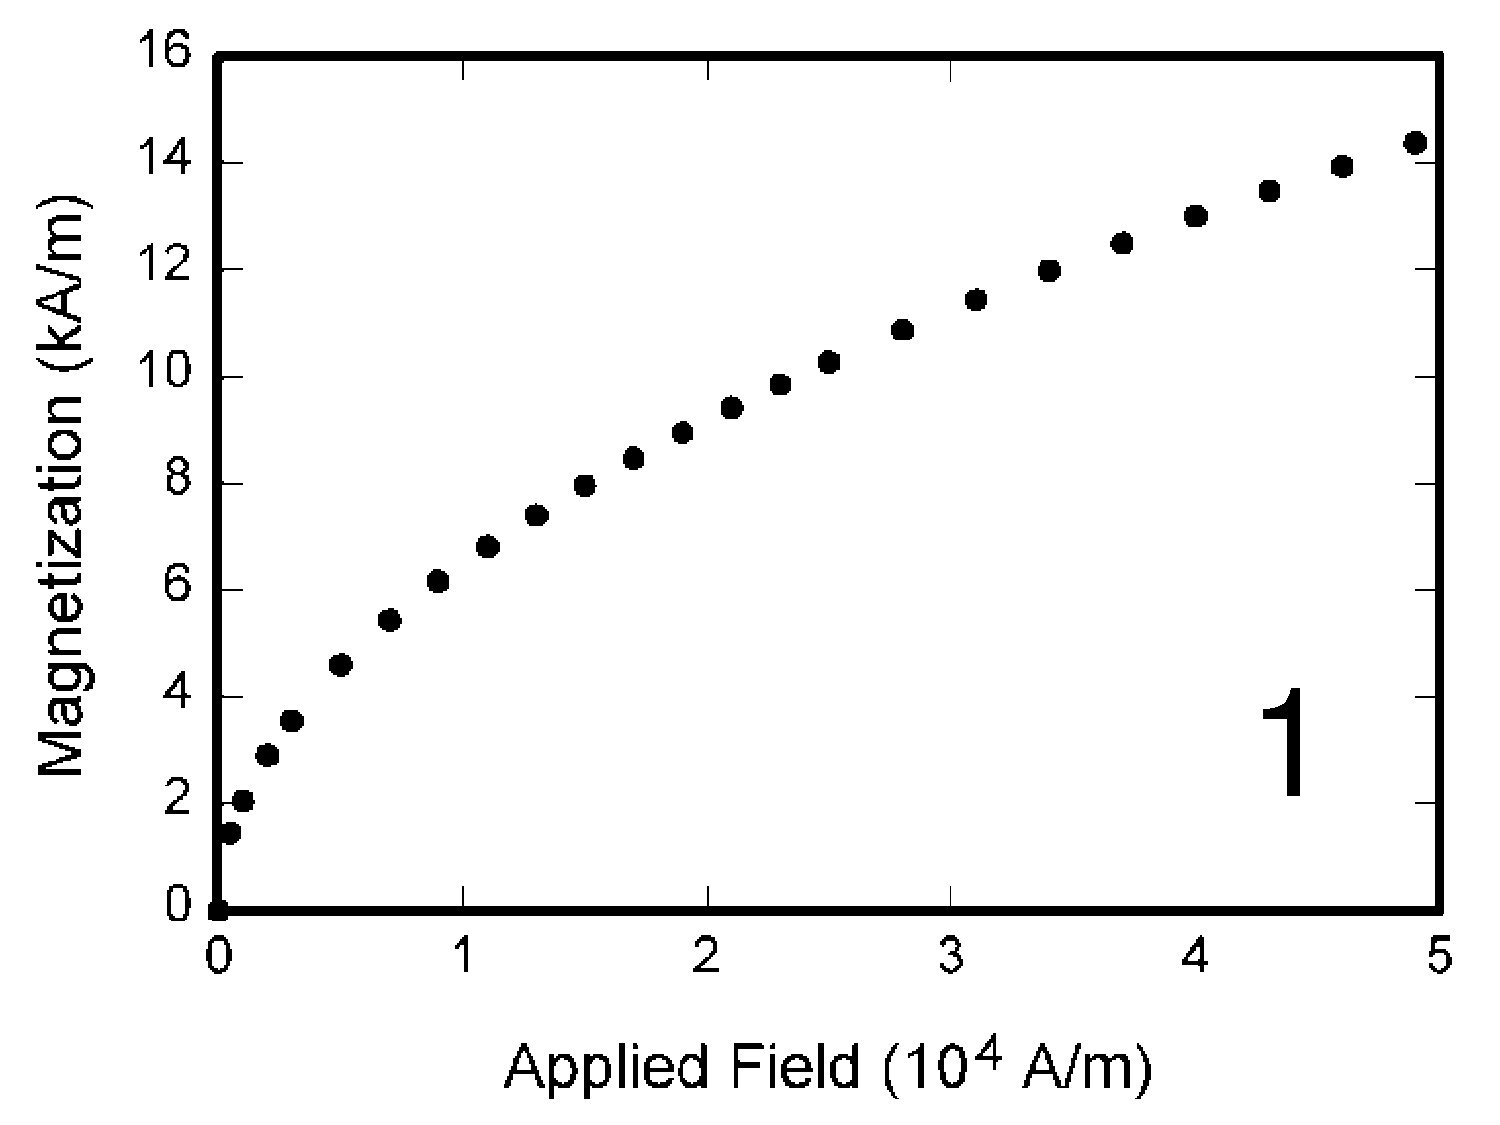
\includegraphics[width=0.8\columnwidth]{Magnetization_vs_Applied_Field_1}%
	\label{fig:2row_by_2col:mag_v_field1}}
	\hfil
	\subfloat[Label of subfigure 2.]{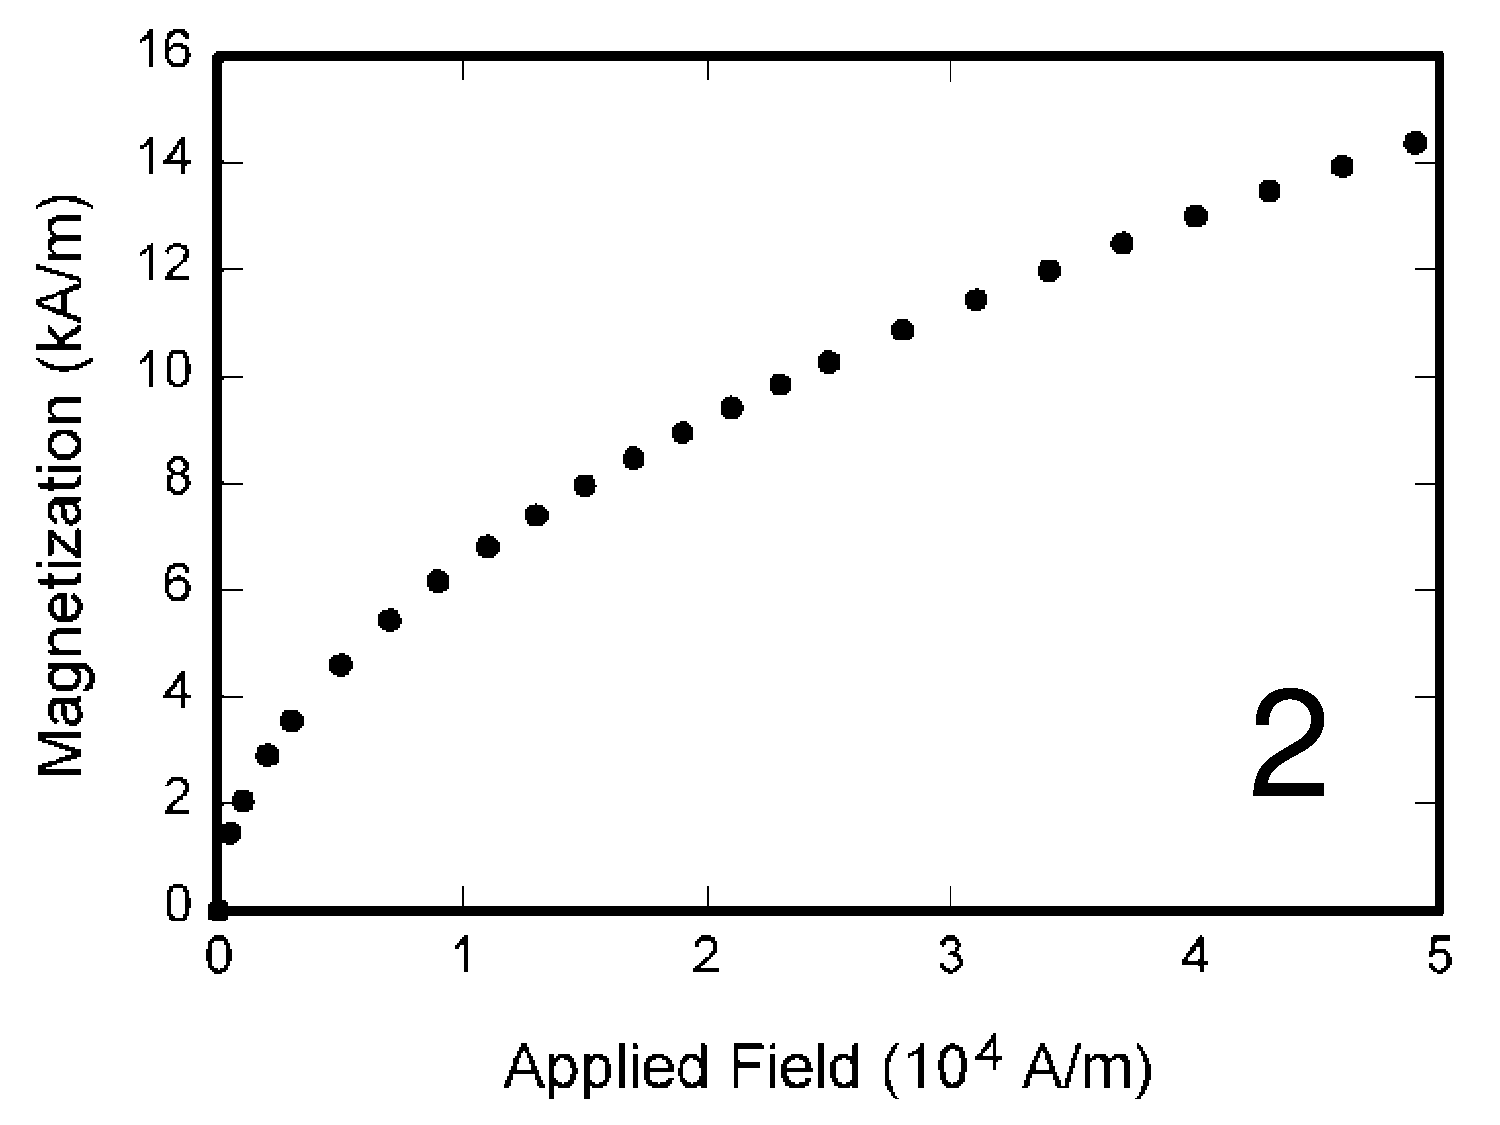
\includegraphics[width=0.8\columnwidth]{Magnetization_vs_Applied_Field_2}%
	\label{fig:2row_by_2col:mag_v_field2}}
	\vfil
	\subfloat[Label of subfigure 3.]{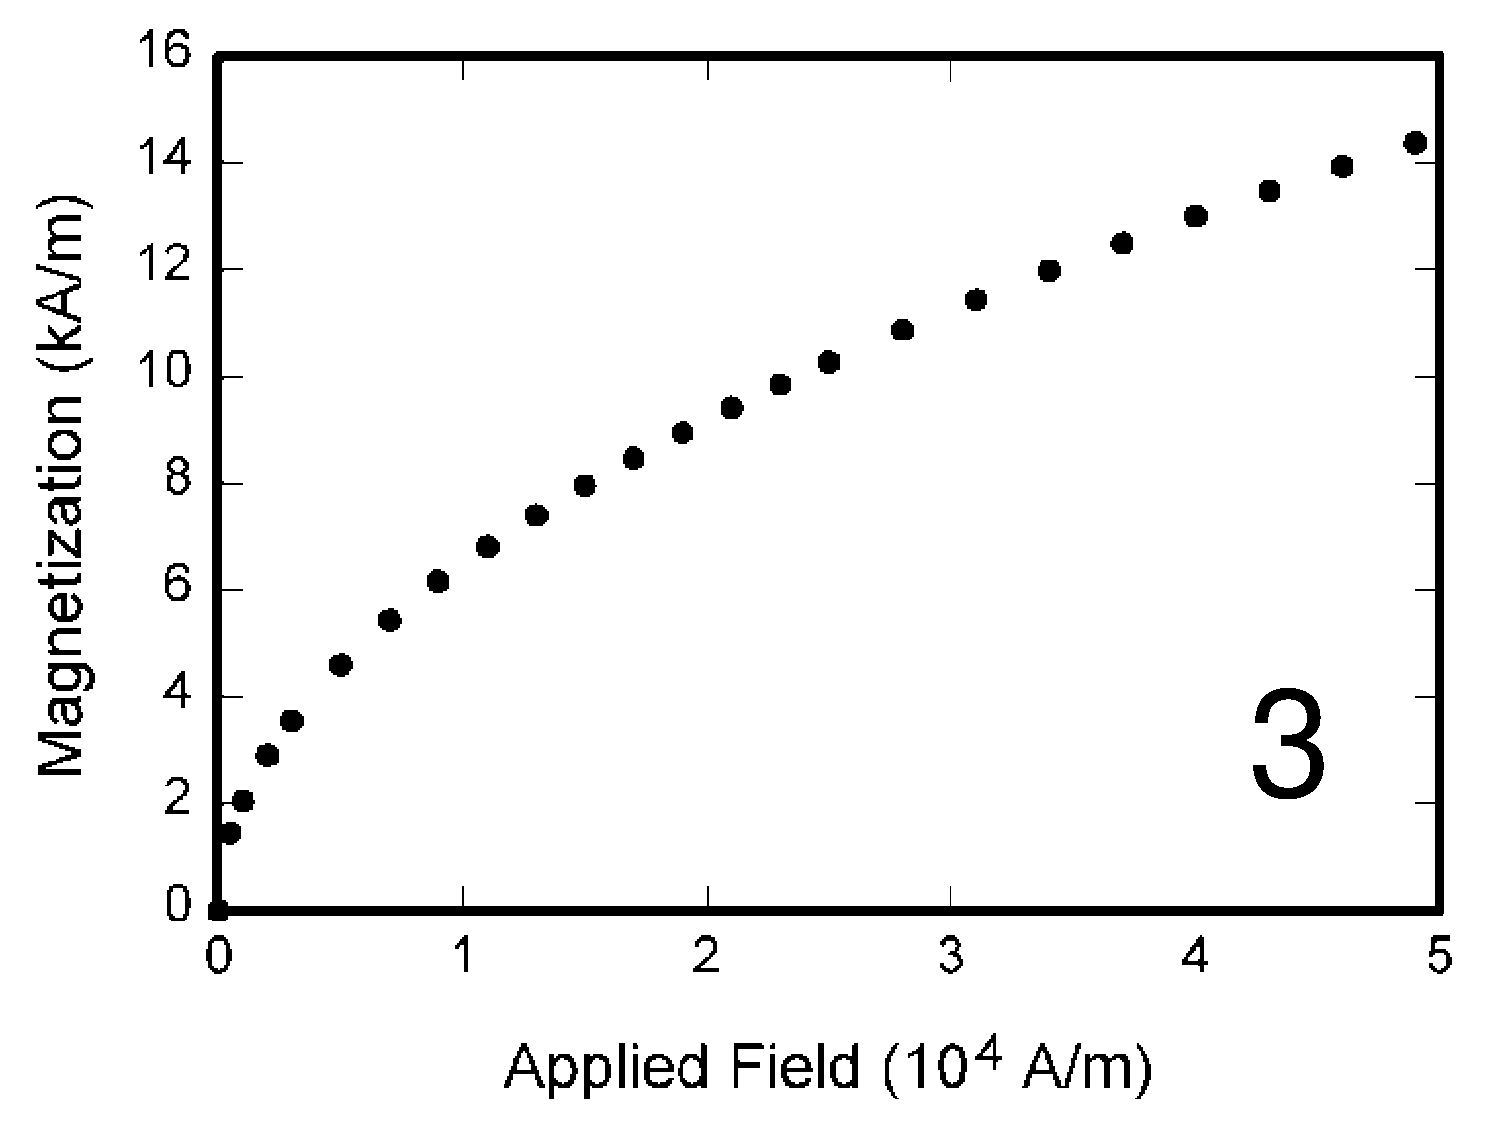
\includegraphics[width=0.8\columnwidth]{Magnetization_vs_Applied_Field_3}%
	\label{fig:2row_by_2col:mag_v_field3}}
	\hfil
	\subfloat[Label of subfigure 4.]{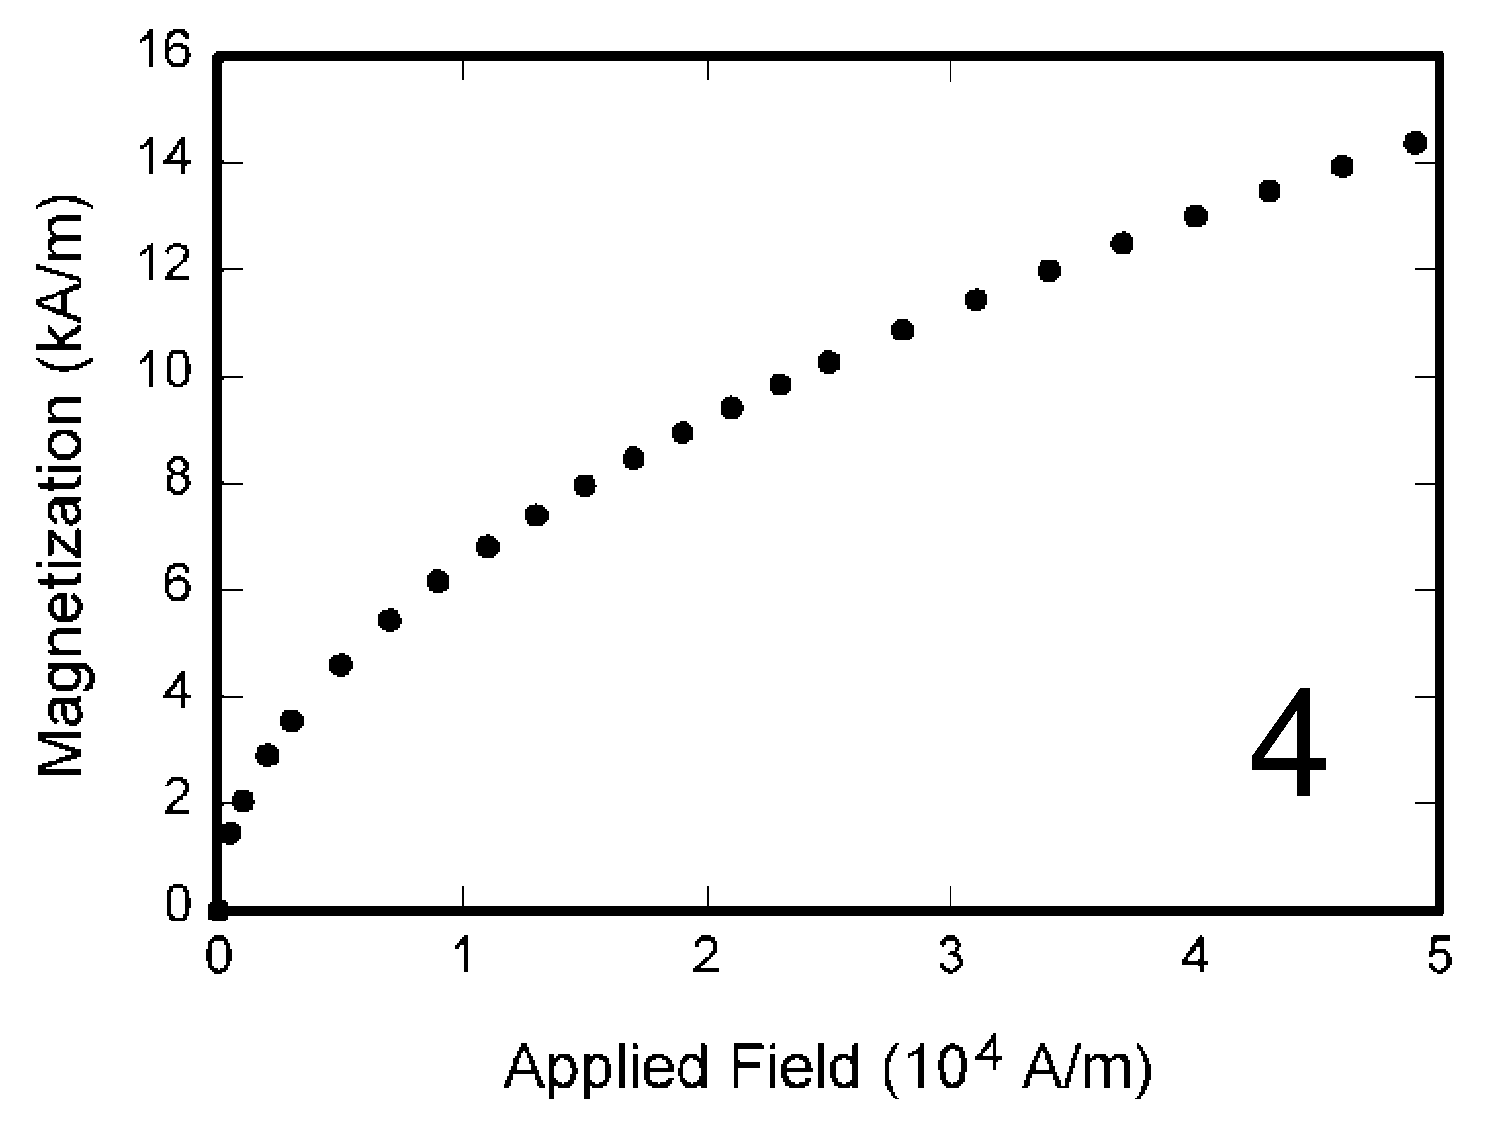
\includegraphics[width=0.8\columnwidth]{Magnetization_vs_Applied_Field_4}%
	\label{fig:2row_by_2col:mag_v_field4}}	
	\caption{Example of four figures in two columns.}
	\label{fig:2row_by_2col}
\end{figure*}



\begin{figure*}[!tb]
	\centering
	\subfloat[Label of subfigure 1.]{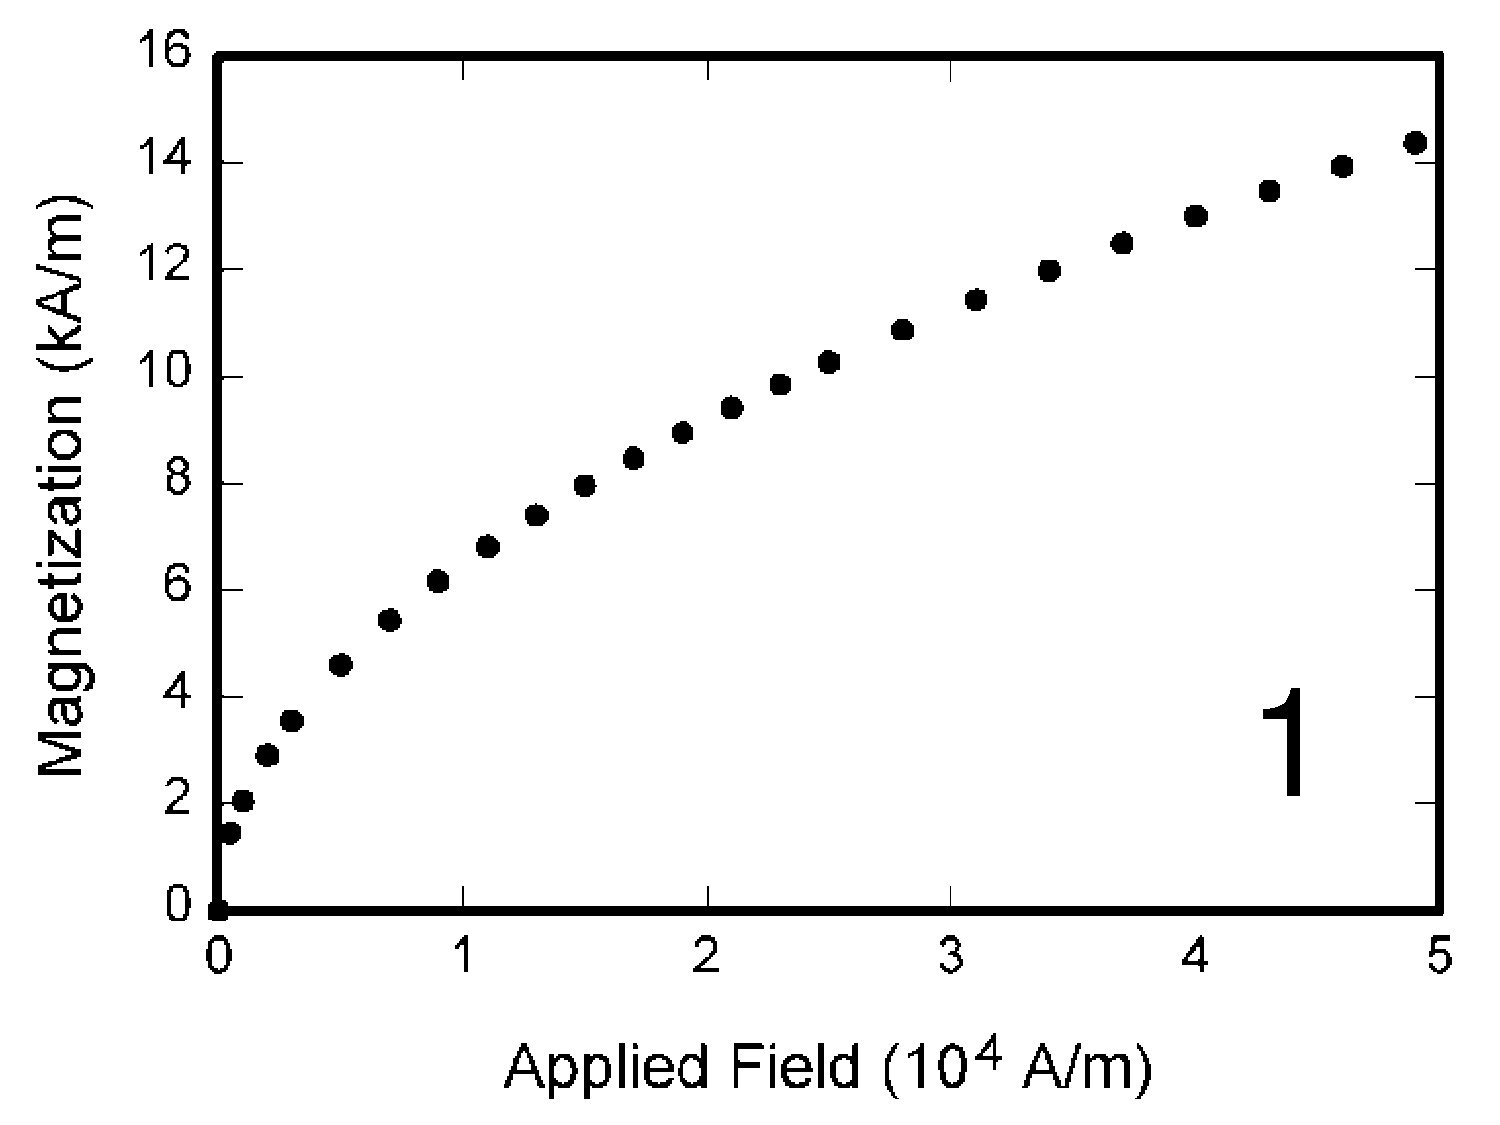
\includegraphics[width=0.45\columnwidth]{Magnetization_vs_Applied_Field_1}%
	\label{fig:1row_by_4col:mag_v_field1}}
	\hfil
	\subfloat[Label of subfigure 2.]{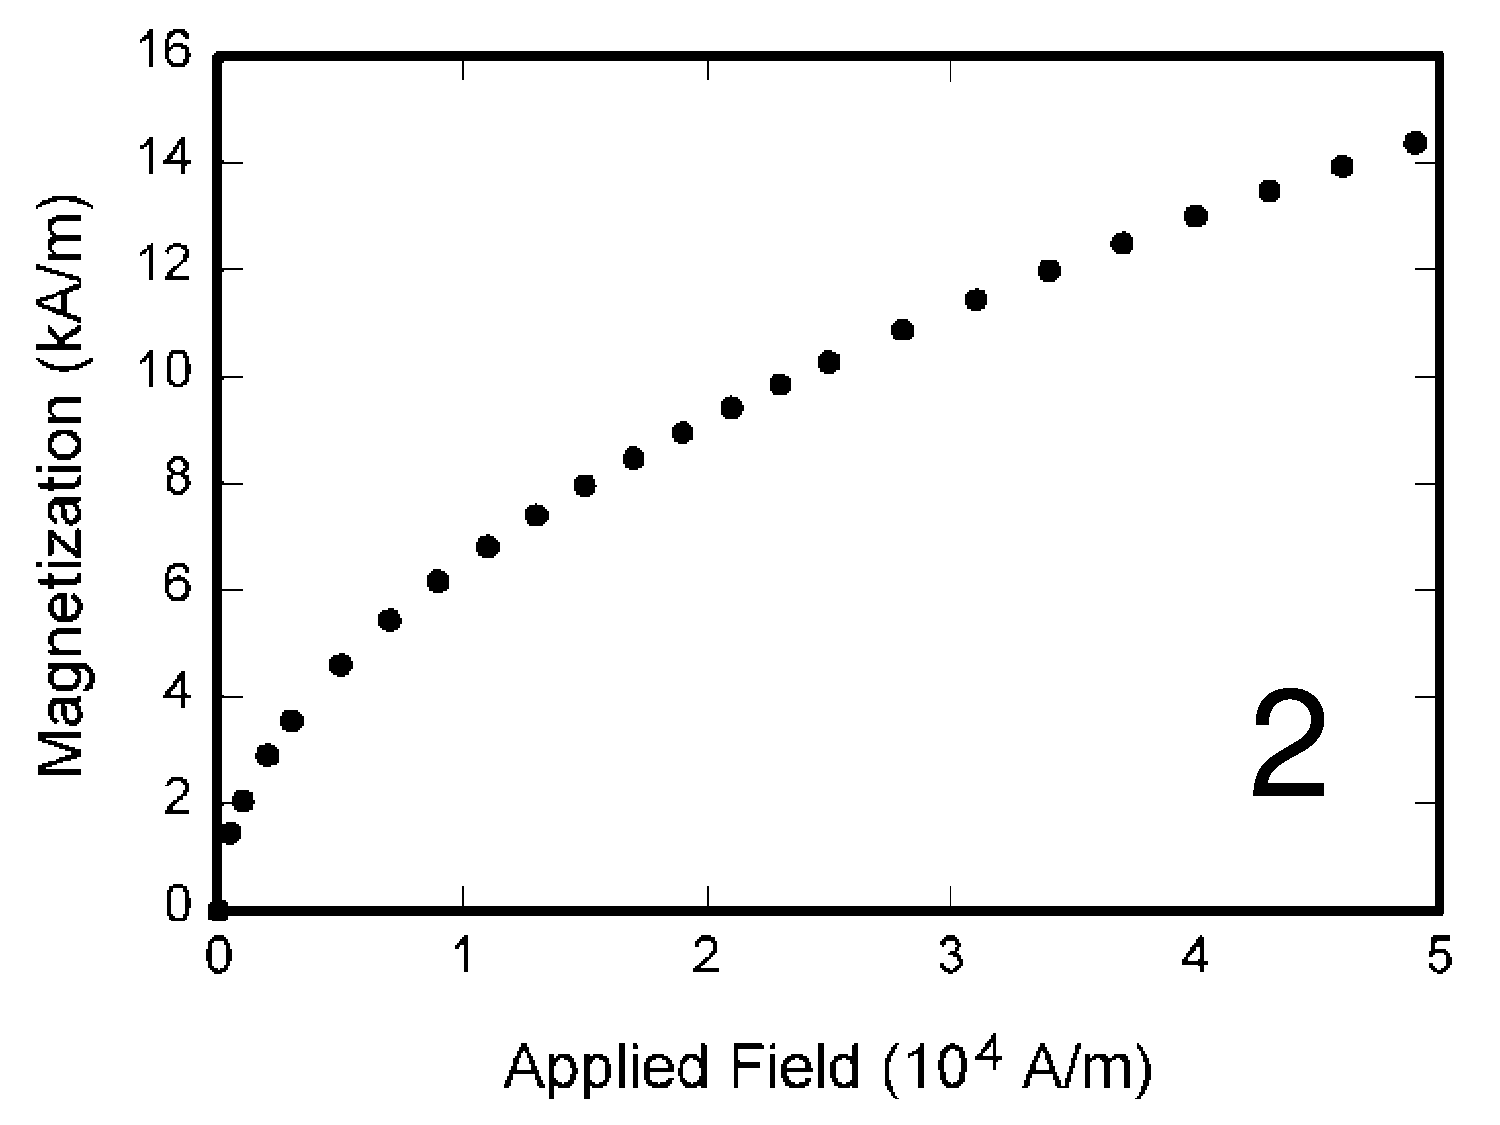
\includegraphics[width=0.45\columnwidth]{Magnetization_vs_Applied_Field_2}%
	\label{fig:1row_by_4col:mag_v_field2}}
	\hfil
	\subfloat[Label of subfigure 3.]{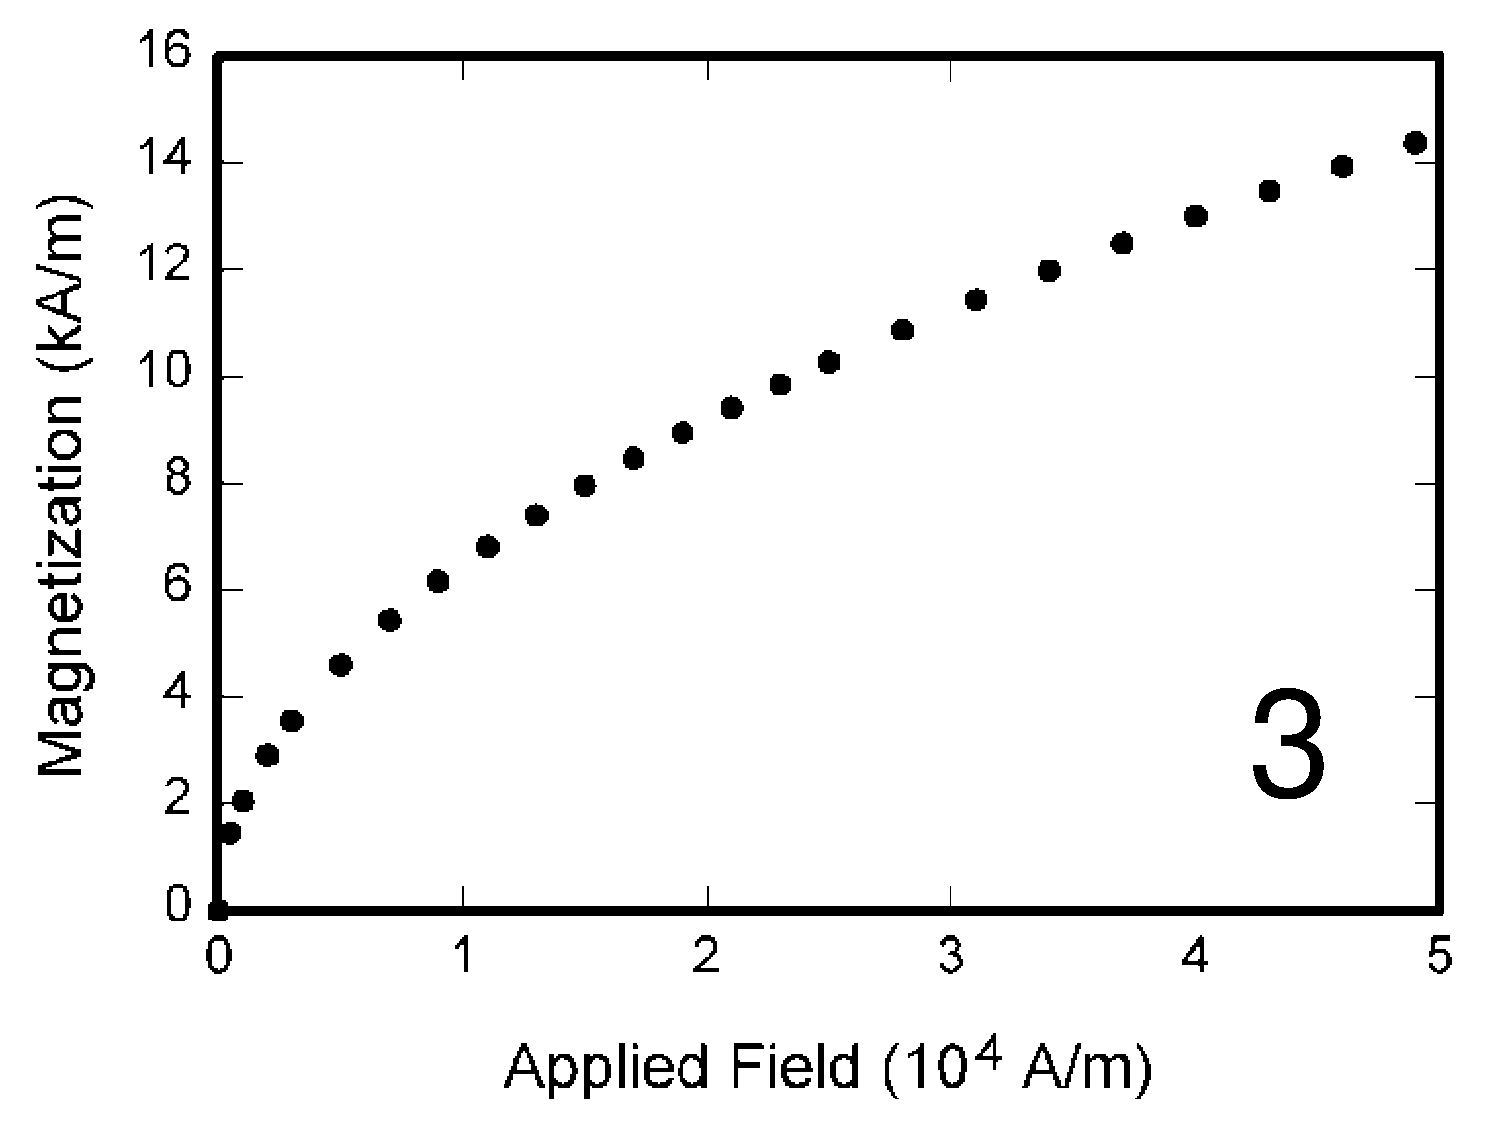
\includegraphics[width=0.45\columnwidth]{Magnetization_vs_Applied_Field_3}%
	\label{fig:1row_by_4col:mag_v_field3}}
	\hfil
	\subfloat[Label of subfigure 4.]{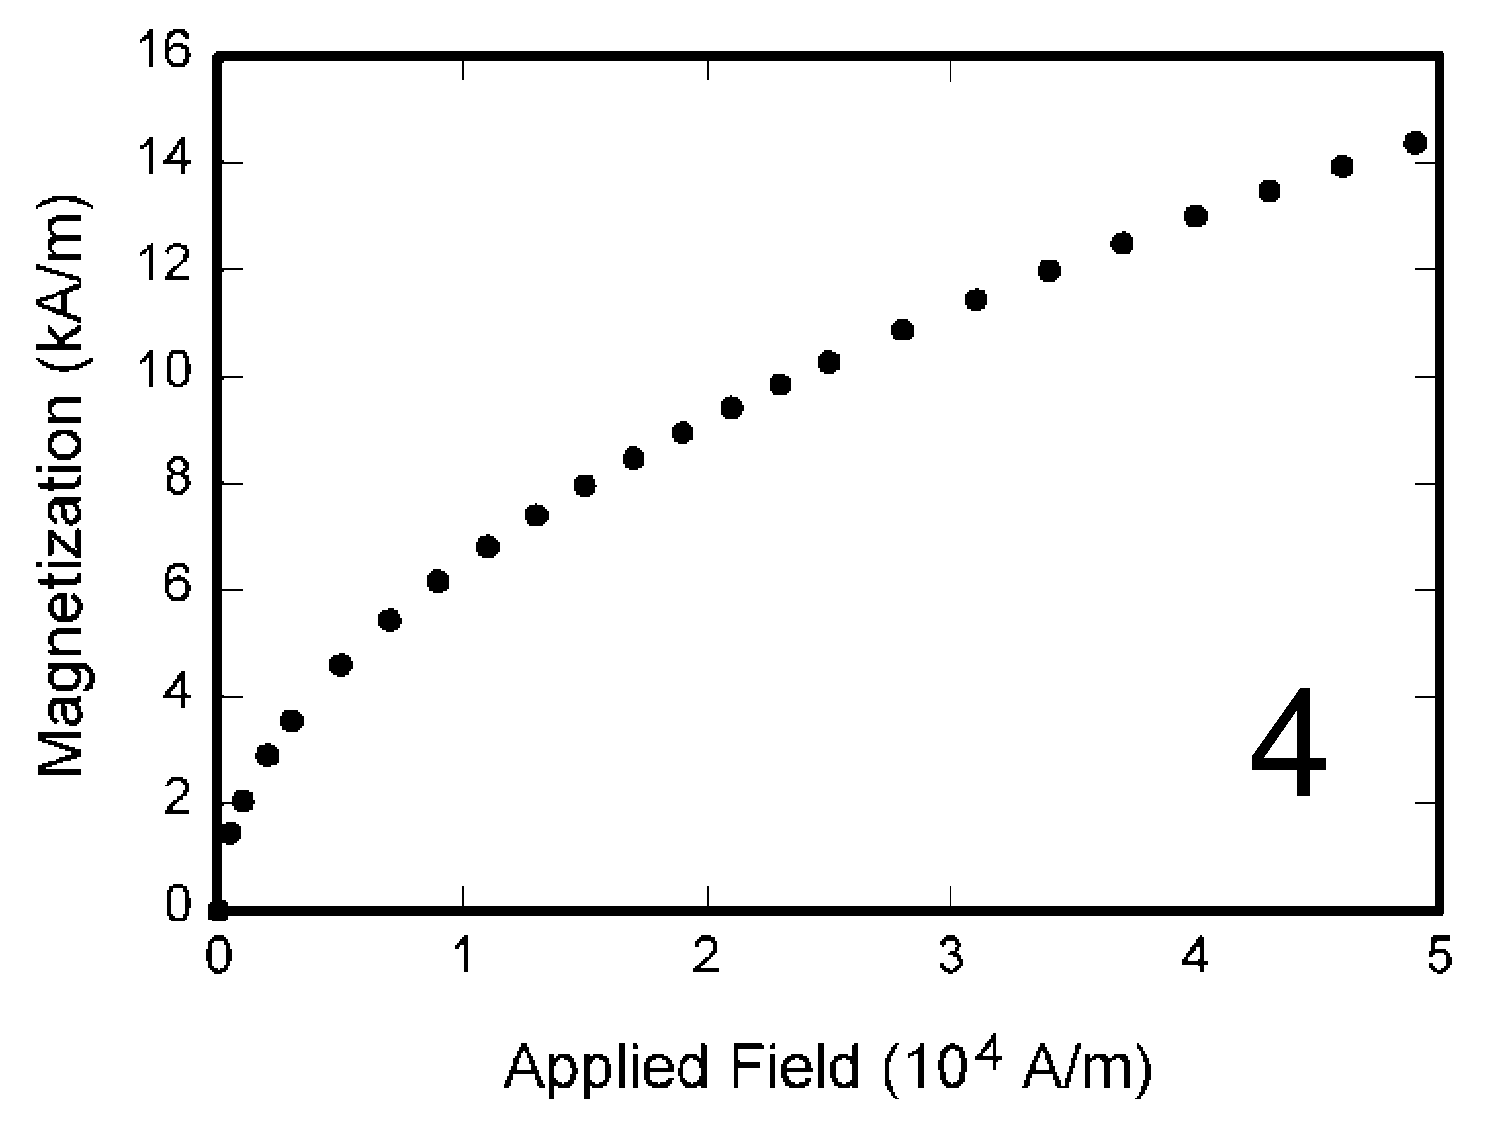
\includegraphics[width=0.45\columnwidth]{Magnetization_vs_Applied_Field_4}%
	\label{fig:1row_by_4col:mag_v_field4}}	
	\caption{Example of four figures in one row.}
	\label{fig:1row_by_4col}
\end{figure*}




\begin{figure}[!tb]
	\centering
	\subfloat[Label of subfigure 1.]{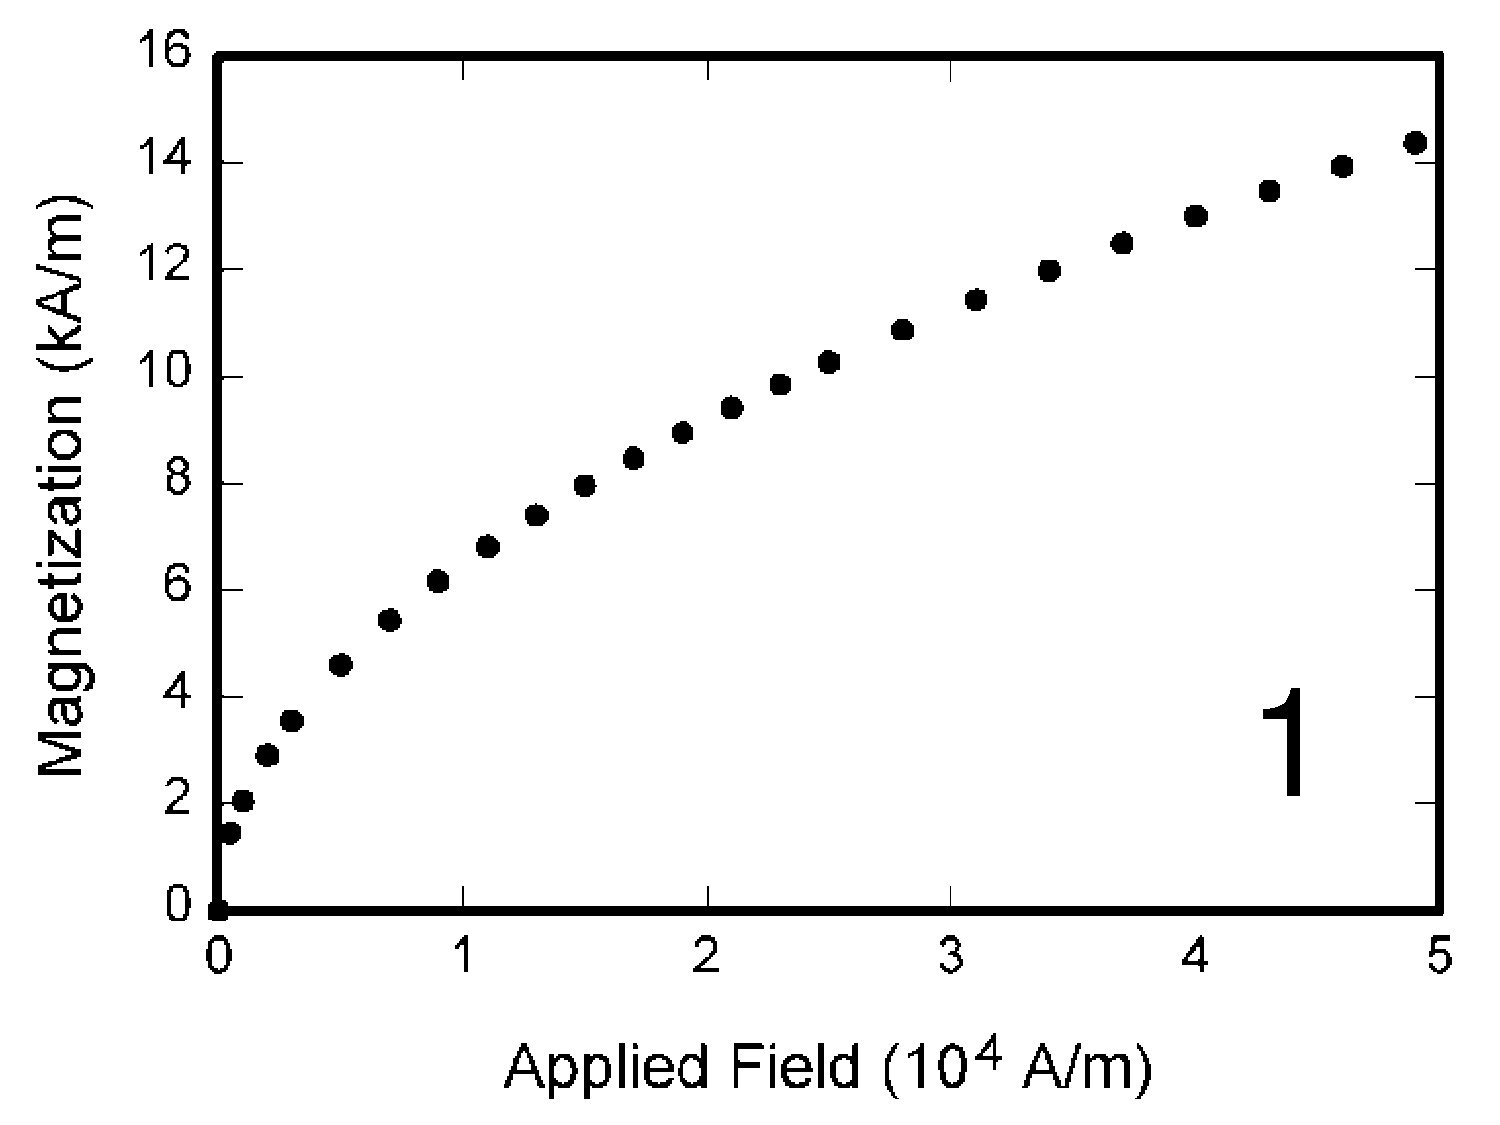
\includegraphics[width=0.7\columnwidth]{Magnetization_vs_Applied_Field_1}%
	\label{fig:4row_by_1col:mag_v_field1}}
	\vfil
	\subfloat[Label of subfigure 2.]{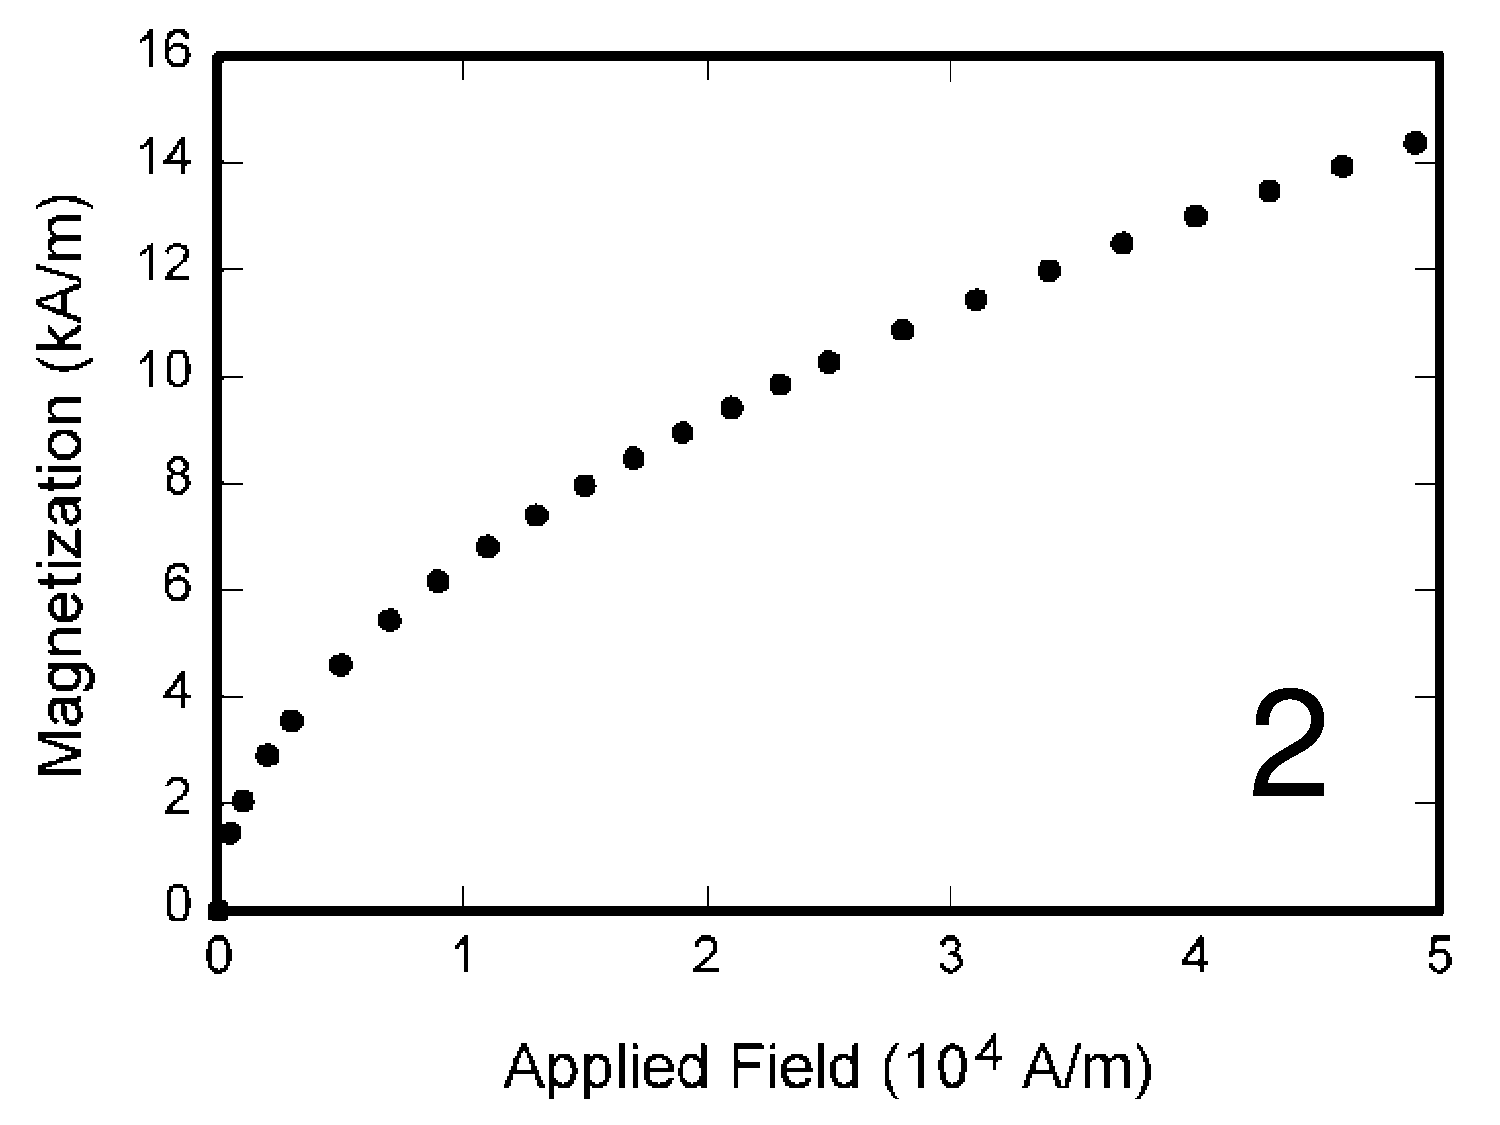
\includegraphics[width=0.7\columnwidth]{Magnetization_vs_Applied_Field_2}%
	\label{fig:4row_by_1col:mag_v_field2}}
	\vfil
	\subfloat[Label of subfigure 3.]{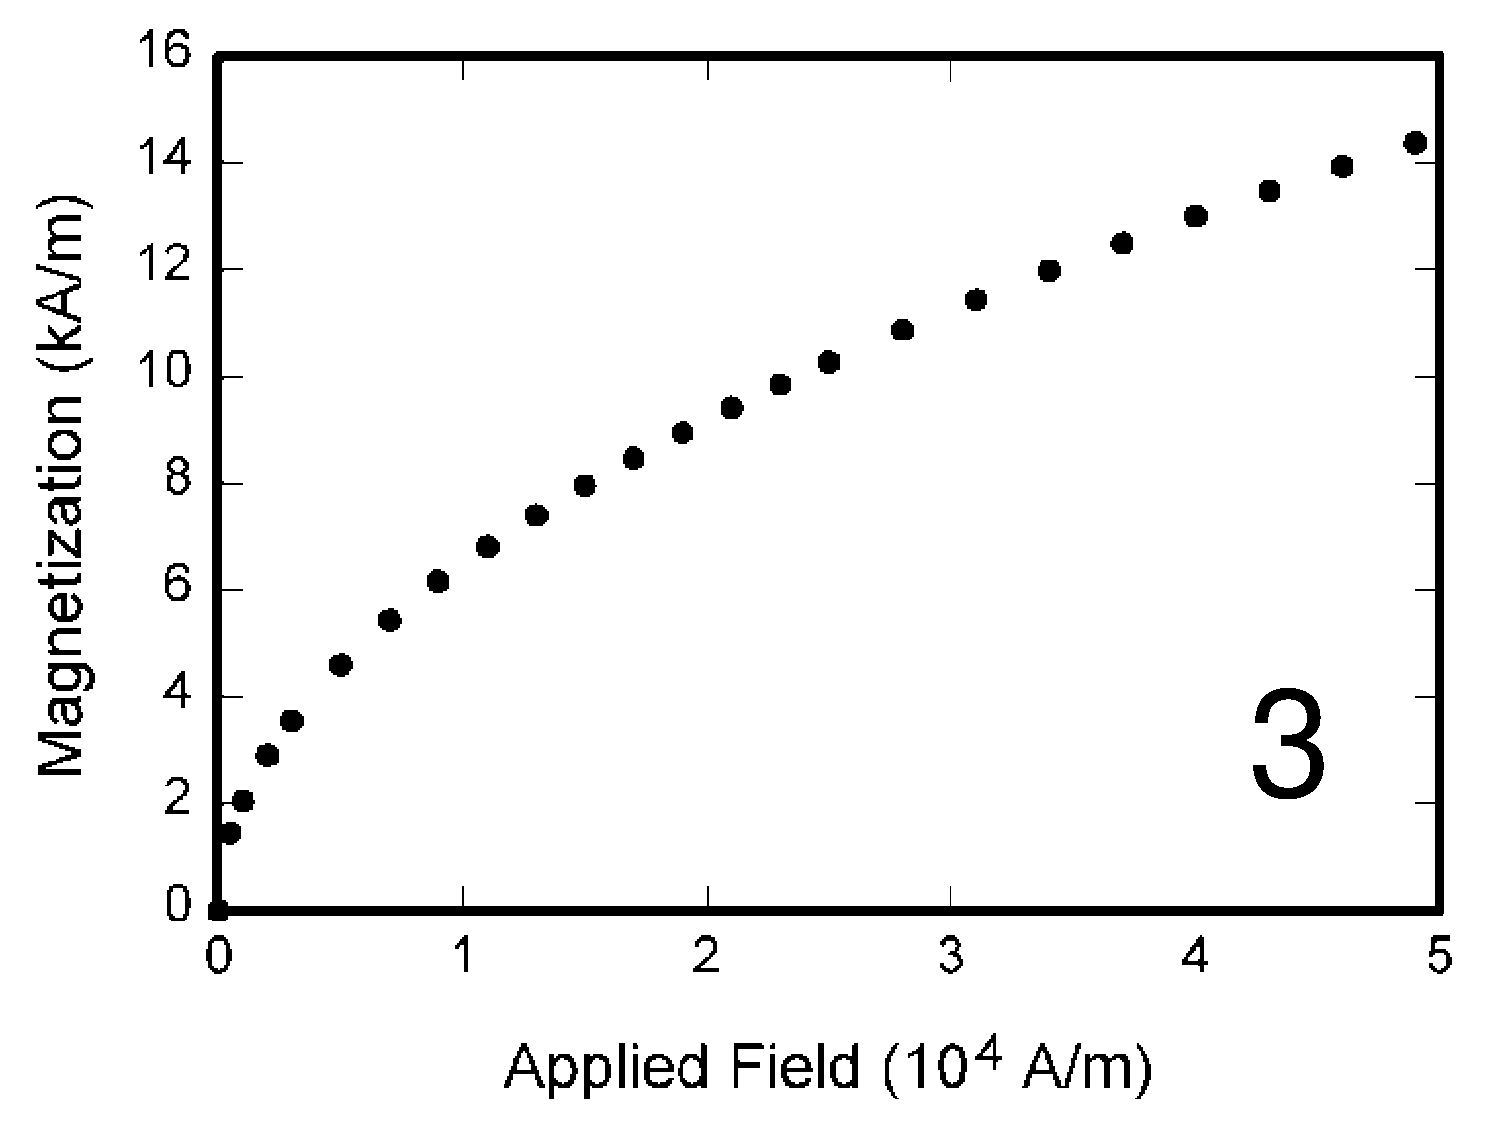
\includegraphics[width=0.7\columnwidth]{Magnetization_vs_Applied_Field_3}%
	\label{fig:4row_by_1col:mag_v_field3}}
	\vfil
	\subfloat[Label of subfigure 4.]{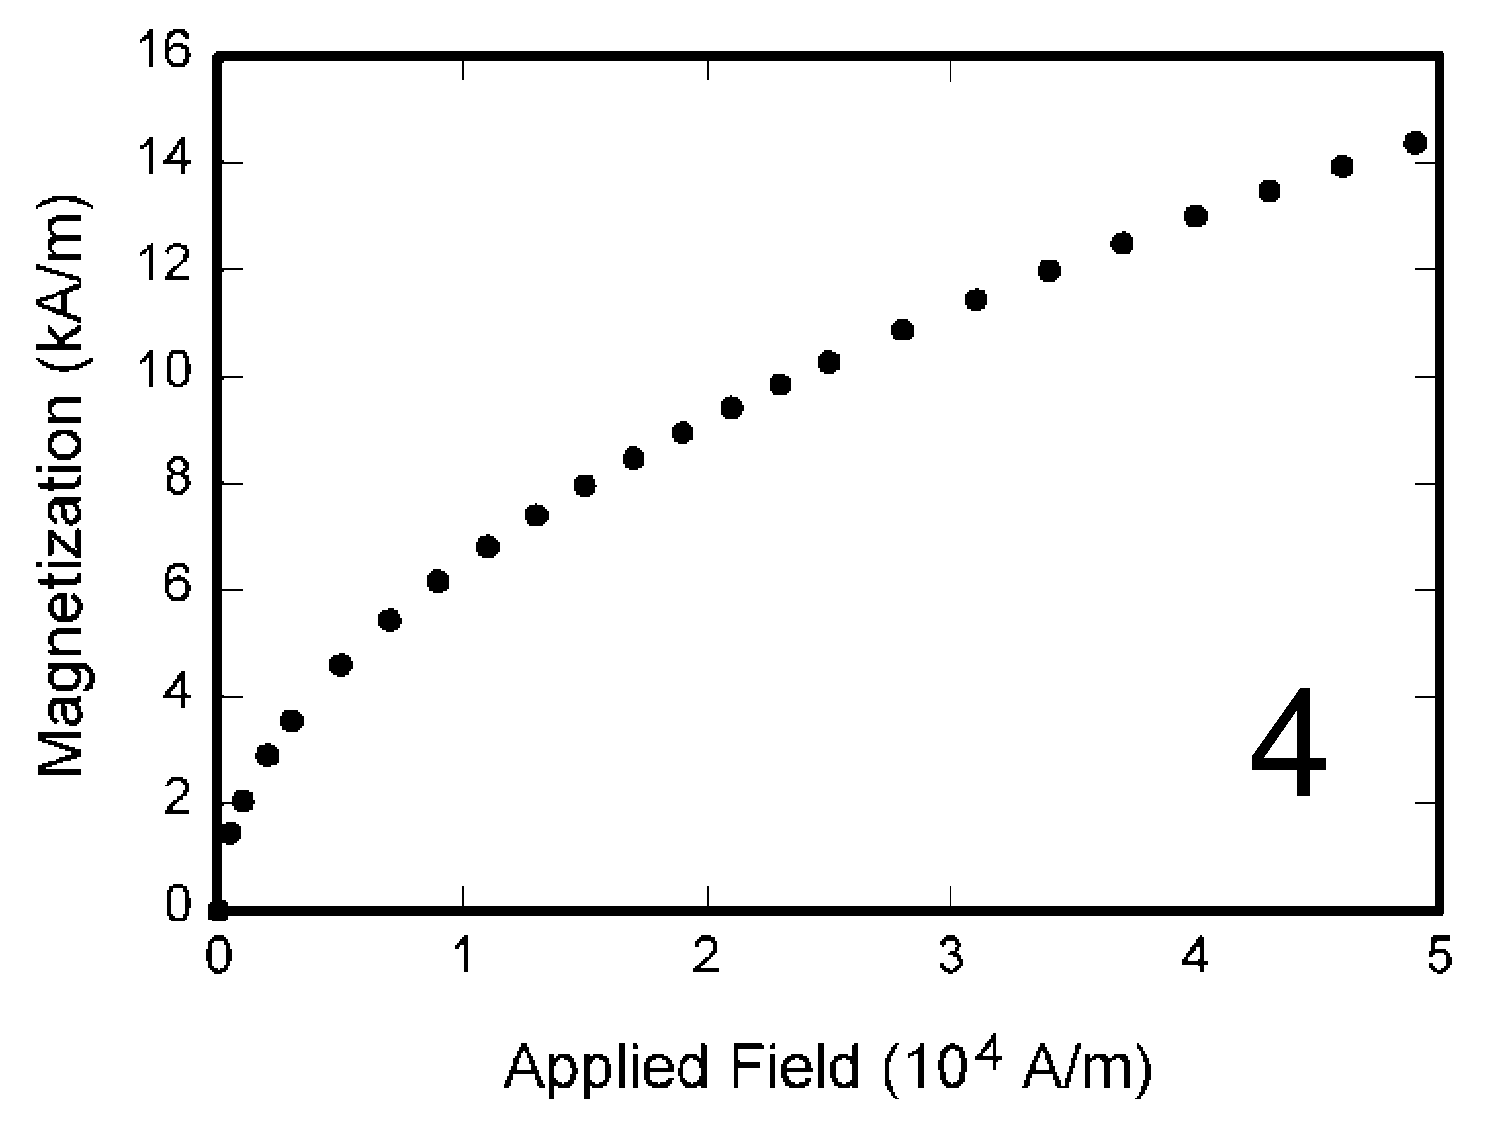
\includegraphics[width=0.7\columnwidth]{Magnetization_vs_Applied_Field_4}%
	\label{fig:4row_by_1col:mag_v_field4}}	
	\caption{Example of four figures in one column.}
	\label{fig:4row_by_1col}
\end{figure}






\subsection{Tables}

\begin{enumerate}
	\item Excel2LaTeX \url{http://www.ctan.org/tex-archive/support/excel2latex/} is suggested as a tool for converting tables made in Excel to LaTeX. 
		
	\begin{enumerate}
		\item If the Excel2LaTeX add-in macro is installed correctly, after making your formatted table in Excel, use the ``Convert Table to \LaTeX'' command in the add-in menu.
		
		\item Uncheck the ``Booktabs-style formatting'' since it is not supported in the template.
		
		\item Copy the Excel2LaTeX windows contents to Clipboard and then paste them in the appropriate location in your \LaTeX\ file.
		
		\item Note that the \verb|\bigstrut| is not supported in this template, so its instances should be erased after pasting the \LaTeX\ Table code in your \LaTeX\ file.
	\end{enumerate}

	\item Note that, for this template, the \verb|\caption| command should come BEFORE the table.
	
	\item Table text will default to \verb|\footnotesize|.  
	
	\item The \verb|\label| must come after \verb|\caption|.
	
	\item Example tables are shown in Tables~\ref{tab:magnetic_properties_units}, \ref{tab:table_example}, and \ref{tab:multi_example}. Table~\ref{tab:two_col} is an example that spans two columns.

\end{enumerate}



\begin{table}[!bt]
	% increase table row spacing, adjust to taste
	\renewcommand{\arraystretch}{1.3}
	\caption{Units for Magnetic Properties~\cite{IEEEMSW2013}}
	\label{tab:magnetic_properties_units}
	\vspace{-2ex}
	\centering
	\scriptsize
 \begin{tabular}{c|c|l}
 \hline
 \hline
 \multirow{2}[2]{*}{Symbol} & \multirow{2}[2]{*}{Quantity} & \multicolumn{1}{c}{Conversion from Gaussian and}\\ 
       &       & \multicolumn{1}{c}{CGS EMU to SI\textsuperscript{a}}\\
 \hline
 \hline
 $\phi$     & magnetic flux & 1 Mx $\rightarrow$ 10\textsuperscript{-8} Wb = 10\textsuperscript{-8} V$\cdot$s\\ \hline
 \multirow{2}[0]{*}{$B$} & magnetic flux density,  & \multirow{2}[0]{*}{1 G $\rightarrow$ 10\textsuperscript{-4} T = 10\textsuperscript{-4} Wb/m\textsuperscript{2}} \\ 
       &   magnetic induction &  \\ \hline
 $H$ & magnetic field strength & 1 Oe $\rightarrow$ 10\textsuperscript{3}/(4$\pi$) A/m \\ \hline
 \multirow{2}[0]{*}{$m$} & \multirow{2}[0]{*}{magnetic moment} & 1 erg/G = 1 emu  \\ 
       &       &   $\rightarrow$ 10\textsuperscript{-3} A$\cdot$m\textsuperscript{2} = 10\textsuperscript{-3} J/T \\ \hline
 \multirow{2}[0]{*}{$M$} & \multirow{2}[0]{*}{magnetization} & 1 erg/(G$\cdot$cm\textsuperscript{3}) = 1 emu/cm\textsuperscript{3} \\ 
       &       &   $\rightarrow$ 10\textsuperscript{3} A/m \\ \hline
 $4\pi M$   & magnetization & 1 G $\rightarrow$ 10\textsuperscript{-8}/(4$\pi$) A/m \\ \hline
 $\sigma$     & specific magnetization & 1 erg/(G $\cdot$ g) = 1 emu/g $\rightarrow$ 1 A$\cdot$m\textsuperscript{2}/kg \\ \hline
 \multirow{2}[0]{*}{$j$} & magnetic dipole  & 1 erg/G = 1 emu  \\ 
       &   moment &   $\rightarrow$ 4p ´ 10\textsuperscript{-10} Wb$\cdot$m \\ \hline
 \multirow{2}[0]{*}{$J$} & \multirow{2}[0]{*}{magnetic polarization} & 1 erg/(G$\cdot$cm\textsuperscript{3}) = 1 emu/cm\textsuperscript{3} \\ 
       &       &   $\rightarrow$ 4$\pi$ ´ 10\textsuperscript{-4} T \\ \hline
 $\kappa$  & susceptibility & 1 $\rightarrow$ 4$\pi$ \\ \hline
 $\kappa_\rho$    & mass susceptibility & 1 cm\textsuperscript{3}/g $\rightarrow$ 4$\pi$ ´ 10\textsuperscript{-3} m\textsuperscript{3}/kg \\ \hline
 \multirow{2}[0]{*}{m} & \multirow{2}[0]{*}{permeability} & 1 $\rightarrow$ 4$\pi$ ´ 10\textsuperscript{-7} H/m  \\ 
       &       &   = 4$\pi$ ´ 10\textsuperscript{-7} Wb/(A$\cdot$m) \\ \hline
 $\mu_\mathrm{r}$    & relative permeability & m $\rightarrow$ mr \\ \hline
$W$ & energy density & 1 erg/cm\textsuperscript{3} $\rightarrow$ 10\textsuperscript{-1} J/m\textsuperscript{3} \\ \hline
$D$  & demagnetizing factor & 1 $\rightarrow$ 1/(4$\pi$)\\
 \hline
 \hline
 \end{tabular}%
\newline
 \begin{tabular}{p{0.9\columnwidth}}
  Vertical lines are optional in tables. Statements that serve as captions for the entire table do not need footnote letters. \\
	\textsuperscript{a}Gaussian units are the same as cg emu for magnetostatics; Mx = maxwell, G = gauss, Oe = oersted; Wb = weber, V = volt, s = second, T = tesla, m = meter, A = ampere, J = joule, kg = kilogram, H = henry.
 \end{tabular}
\end{table}






\begin{table}[!bt]
	% increase table row spacing, adjust to taste
	\renewcommand{\arraystretch}{1.3}
	\caption{An Example of a Table}
	\label{tab:table_example}
	\vspace{-2ex}
	\centering
	% Some packages, such as MDW tools, offer better commands for making tables
	% than the plain LaTeX2e tabular which is used here.
	\begin{tabular}{c|c}
		\hline
		\hline
		One & Two\\
		\hline
		Three & Four\\
		\hline
		\hline
	\end{tabular}
\end{table}



\begin{table}[!bt]
	% increase table row spacing, adjust to taste
	\renewcommand{\arraystretch}{1.3}
	\caption{A Multicolumn and Multirow Table Example}
	\label{tab:multi_example}
	\vspace{-2ex}
	\centering
 \begin{tabular}{c|c|c|c}
 \hline
\hline
 \multicolumn{2}{c|}{\textbf{T1}} & \multicolumn{2}{|c}{\textbf{T2}} \\
 \hline
 \textit{Player} & \textit{AFG} & \textit{Player} & \textit{AFG} \\
 \hline
 T1P1 & \multirow{2}[4]{*}{30} & T2P3 & 30 \\
\cline{1-1}\cline{3-4} T1P2 &       & T2P2 & 20 \\
 \hline
 T1P3  & 15    & T2P3  & 15 \\
 \hline
 \hline
 \end{tabular}%
\end{table}




\begin{table*}[!bt]
	% increase table row spacing, adjust to taste
	\renewcommand{\arraystretch}{1.3}
	\caption{Example of a Table Occupying Two Columns. Eigenvalues (a.u.) of $n=3,4$ states of Confined ECSC Potential for $\delta=0.02$ (numbers in the parentheses denote reference energies quoted from \cite{Lumb2014})}
	\label{tab:two_col}
	\vspace{-2ex}
	\centering
	\scriptsize	
	
	\begin{tabular}{c | c | c | c | c | c}
		\hline
		\hline
		State  & $r_c=0.1$   &  $r_c=0.5$    &   $r_c=1$     &  $r_c=2$            &   $r_c=5$            \\
		\hline
		$3s$   & 4406.1416518  & 170.60516396    & 40.883123723     & 9.3341469004      & 1.0731978420      \\
				   &               &                 &                  & (9.33415)         & (1.07320)         \\ 
		$3p$   & 2960.4823022  & 114.66355228    & 27.493994384     & 6.2889991502      & 0.7276959975      \\
					 &               &                 &                  & (6.28900)         & (0.72770)         \\ 
		$3d$   & 1644.5499223  & 63.180184177    & 14.987462939     & 3.3475046681      & 0.3490909625      \\
					 &               &                 &                  & (3.34750)         & (0.34909)         \\ 
		$4s$   & 7857.6491849  & 308.21724725    & 75.150492179     & 17.836089963      & 2.4023028763      \\
					 &               &                 &                  & (17.83609)        & (2.40230)         \\ 
		$4p$   & 5918.2028888  & 232.44795983    & 56.778032985     & 13.530580567      & 1.8504011627      \\
					 &               &                 &                  & (13.53058)        & (1.85040)         \\ 
		$4d$   & 4115.6026320  & 161.37700634    & 39.335318864     & 9.3341465110      & 1.2596272053      \\
					 &               &                 &                  & (9.33415)         & (1.25963)         \\ 
		$4f$   & 2426.4155489  & 94.646597432    & 22.915824203     & 5.3620893411      & 0.6894218988      \\
			 		 &               &                 &                  & (5.36209)         & (0.68942)         \\ 
		\hline
					 & $r_c=10$       &   $r_c=20$      &     $r_c=30$     &   $r_c=50$       &  $r_c=100$        \\
		\hline
		$3s$   & 0.1113277900   & $-$0.0302492345 & $-$0.0358787689  & $-$0.0360250925  & $-$0.0360251051   \\
					 & (0.11133)      &                 &                  & ($-$0.03603)     &                   \\
		$3p$   & 0.0691008416   & $-$0.0319140038 & $-$0.0358733580  & $-$0.0359675961  & $-$0.0359676034   \\
					 & (0.06910)      &                 &                  & ($-$0.03597)     &                   \\
		$3d$   & 0.0128160637   & $-$0.0342064512 & $-$0.0358194164  & $-$0.0358506603  & $-$0.0358506623   \\
					 & (0.01282)      &                 &                  & ($-$0.03585)     &                   \\
		$4s$   & 0.4250635505   & 0.0363462881    & $-$0.0054277289  & $-$0.0124953824  & $-$0.0125717772   \\
					 & (0.42506)      &                 &                  & ($-$0.01250)     &                   \\
		$4p$   & 0.3359680167   & 0.0277302857    & $-$0.0066764629  & $-$0.0124281276  & $-$0.0124857523   \\
					 & (0.33597)      &                 &                  & ($-$0.01243)     &                   \\
		$4d$   & 0.2223514916   & 0.0141166051    & $-$0.0086778605  & $-$0.0122798641  & $-$0.0123102664   \\
					 & (0.22235)      &                 &                  & ($-$0.01228)     &                   \\
		$4f$   & 0.1081309850   & $-$0.0003604550 & $-$0.0106312256  & $-$0.0120295162  & $-$0.0120381878   \\
					 & (0.10813)      &                 &                  & ($-$0.01203)     &                   \\
		\hline	
		\hline		
	\end{tabular}
			
\end{table*}


%
%\begin{table}
%\caption {\label{tab:table4} Eigenvalues (a.u.) of $n=3,4$ states of confined ECSC potential for 
%$\delta=0.02$. Numbers in the parentheses denote reference energies quoted from \cite{lumb14}.} 
%
%\end{table}

















\section{Equation Examples}

\begin{enumerate}
	\item It is to be noted that~\cite{ISO800002} and its updates shall be used as the standard for typesetting maths like equations, variables, etc. 
	
	\begin{description}
			For example, the derivative of $f \left( x \right)$ with respect to $x$ is written as $\mathrm{d} f \left( x \right)/\mathrm{d} x$.  Note that $\mathrm{d}$ is not italicized according to~\cite{ISO800002}.   
	\end{description}
		
	\item EqualX and its online counterparts like \url{https://www.codecogs.com/latex/eqneditor.ph} are utilities that can be used by beginners in typesetting math in \LaTeX. 
	
	\item A compiled resource of typesetting math in \LaTeX\ can be found in \url{http://en.wikipedia.org/wiki/Help:Displaying_a_formula}. 

	\item In \LaTeX\, inline equations/math are enclosed inside \verb|$ $| delimiters, e.g. \verb|$x_\mathrm{pos}^{-\sqrt{n}}$|, which produces $x_\mathrm{pos}^{-\sqrt{n}}$.  
	
	\item Displayed equations should be numbered and is handled by \LaTeX\ when using the \texttt{eqnarray} environment (and similar).
	
	\item Examples are shown below. 


  In~\eqref{eq:conv}, the output signal $y\left( t \right) $ is the result of the convolution of the input signal $x\left( t \right) $ 
and the impulse response $h\left( t \right) $.

\begin{eqnarray}   
     y\left( t \right) = h\left( t \right) * x\left( t \right)=\int_{-\infty}^{+\infty}h\left( t-\tau \right)x\left( \tau \right) \mathrm{d}\tau
	\label{eq:conv}
\end{eqnarray}






\begin{eqnarray}
	\left[ \dfrac{ V_{1} }{ I_{1} } \right] = 
	\begin{bmatrix}
		A & B \\ 
		C & D 
	\end{bmatrix} 
	\left[ \dfrac{ V_{2} }{ I_{2} } \right]
	\label{eq:ABCD}
\end{eqnarray}






\begin{eqnarray}
\dfrac{1}{2} < \left\lfloor \mathrm{mod}\left(\left\lfloor \dfrac{y}{17} \right\rfloor 2^{-17 \lfloor x \rfloor - \mathrm{mod}(\lfloor y\rfloor, 17)},2\right)\right\rfloor
\label{eq:rn}
\end{eqnarray}




	\item To make your equations more compact, you may use the solidus ( / ), the exponential function, or appropriate exponents.

	\item  Use parentheses to avoid ambiguities in denominators. 
	
	\item Punctuate equations when they are part of a sentence, as in

\setlength{\arraycolsep}{0.0em}
\begin{eqnarray}
\int_0^{r_2} F \left(r, \phi \right) \mathrm{d}r \mathrm{d} \phi &{} = {}&  
\left[\sigma r_2 / \left( 2 \mu_0 \right) \right] \cdot \nonumber\\
&& \hspace{-6em} \int_0^\infty \exp 
\left(-\lambda \left| z_j - z_i  
\right| \right) \lambda^{-1} 
J_1 \left( \lambda r_2 \right)
J_0 \left( \lambda r_1 \right) 
\mathrm{d}\lambda .
\label{eq:besld}
\end{eqnarray}
\setlength{\arraycolsep}{5pt}

 Notice that \eqref{eq:besld} is part of the sentence that just ended, thus the sentence ends in a period.

	\item Be sure that the symbols in your equation have been defined before the equation appears or immediately following. Italicize symbols (\textit{T} might refer to temperature, but T is the unit tesla). 
	
	\item Refer to ``(1),'' not ``Eq. (1)'' or ``equation (1),'' except at the beginning of a sentence: ``Equation~(1) is ... .''

\end{enumerate}














\section{Typography, Semantics, and Syntax-Related Instructions~That Need Emphasis}

\subsection{Abbreviations, Acronyms, and Units}

\begin{enumerate}
	\item  Define abbreviations and acronyms the first time they are used in the text, even after they have already been defined in the abstract. 
	
	\item Abbreviations that incorporate periods should not have spaces: write ``C.N.R.S.,'' not ``C. N. R. S.'' 
	
	\item Do not use abbreviations in the title unless they are unavoidable.

	\item Use either SI (MKS) or CGS as primary units. (SI units are strongly encouraged.) 
	
	\begin{enumerate}
		\item English units may be used as secondary units (in parentheses). 
	
		\item For example, write ``15 Gb/cm\textsuperscript{2} (100 Gb/in\textsuperscript{2}).'' 
		
		\item An exception is when English units are used as identifiers in trade, such as ``3.5-in disk drive.'' 
		
		\item Avoid combining SI and CGS units, such as current in amperes and magnetic field in oersteds. This often leads to confusion because equations do not balance dimensionally. If you must use mixed units, clearly state the units for each quantity in an equation.

		\item The SI unit for magnetic field strength $H$ is A/m. However, if you wish to use units of T, either refer to magnetic flux density B or magnetic field strength symbolized as $\mu_0 H$. 
		
		\end{enumerate}
		
	\item Use the center dot to separate compound units, e.g., ``A~$\cdot$~m\textsuperscript{2}.''
	
\end{enumerate}




\subsection{Some Related Technical Writing Instructions}

\begin{enumerate}
	\item Document titles should be written in uppercase and lowercase letters, not all uppercase.
	
	\item Avoid writing long formulas with subscripts in the title; short formulas that identify the elements are fine (e.g., ``Nd–Fe–B''). 
	
	\item Given that table captions serve much like titles, are usually capitalized except for words such as a, an, and, as, at, but, by, for, in, nor, of, on, or, the, to, and up, which are usually not capitalized unless they are the first or last word of the caption. 
	
	\item Use one space after periods and colons.
	
	\item Hyphenate complex modifiers: ``zero-field-cooled magnetization.'' 
	
	\item Avoid dangling participles, such as, ``Using (1), the potential was calculated.'' [It is not clear who or what used (1).] Write instead, ``The potential was calculated by using (1),'' or ``Using (1), we calculated the potential.'' 
	
	\item Use a zero before decimal points: ``0.25,'' not ``.25.'' 
	
	\item Use ``cm\textsuperscript{3},'' not ``cc.'' 
	
	\item Indicate sample dimensions as ``0.1~cm $\times$ 0.2~cm,'' not ``0.1~$\times$~0.2 cm\textsuperscript{2}.'' 
	
	\item The abbreviation for ``seconds'' is ``s,'' not ``sec.'' 
	
	\item Use ``Wb/m\textsuperscript{2}'' or ``webers per square meter,'' not ``webers/m\textsuperscript{2}.'' 
	
	\item When expressing a range of values, write ``7 to 9'' or ``7-9,'' not ``7$\sim$9.''

	\item A parenthetical statement at the end of a sentence is punctuated outside of the closing parenthesis (like this). (A parenthetical sentence is punctuated within the parentheses.) 
	
	\item In American English, periods and commas are within quotation marks, like ``this period.'' Other punctuation is ``outside''! 
	
	\item Avoid contractions; for example, write ``do not'' instead of ``don't.'' 
	
	\item The serial comma is preferred: ``A, B, and C'' instead of ``A, B and C.'' 
	
	\item \emph{\rdfnt{In most technical, scientific, and academic documents, the third-person writing point of view is used}}. 
	
	\item Remember to check spelling. 

\end{enumerate}




\subsection{Some Common Mistakes}
\begin{enumerate}
	\item The word ``data'' is plural, not singular. 
	
	\item The subscript for the permeability of vacuum $\mu_0$ is zero, not a lowercase letter ``o.''
	
	\item The term for residual magnetization is ``remanence''; the adjective is ``remanent''; do not write ``remnance'' or ``remnant.'' 
	
	\item Use the word ``micrometer'' instead of ``micron.'' 
	
	\item A graph within a graph is an ``inset,'' not an ``insert.'' 
	
	\item The word ``alternatively'' is preferred to the word ``alternately'' (unless you really mean something that alternates). 
	
	\item Use the word ``whereas'' instead of ``while'' (unless you are referring to simultaneous events). 
	
	\item Do not use the word ``essentially'' to mean ``approximately'' or ``effectively.'' Do not use the word ``issue'' as a euphemism for ``problem.'' 
	
	\item When compositions are not specified, separate chemical symbols by en-dashes; for example, ``NiMn'' indicates the intermetallic compound Ni\textsubscript{0.5}Mn\textsubscript{0.5} whereas ``Ni–Mn'' indicates an alloy of some composition Ni\textsubscript{x}Mn\textsubscript{1-x}.

	\item Be aware of the different meanings of the homophones ``affect'' (usually a verb) and ``effect'' (usually a noun), ``complement'' and ``compliment,'' ``discreet'' and ``discrete,'' ``principal'' (e.g., ``principal investigator'') and ``principle'' (e.g., ``principle of measurement''). 
	
	\item Do not confuse ``imply'' and ``infer.'' 

	\item Prefixes such as ``non,'' ``sub,'' ``micro,'' ``multi,'' and ``ultra'' are not independent words; they should be joined to the words they modify, usually without a hyphen. 
	
	\item There is no period after the ``et'' in the Latin abbreviation ``et al.'' (it is also italicized). 
	
	\item The abbreviation ``i.e.,'' means ``that is,'' and the abbreviation ``e.g.,'' means ``for example'' (these abbreviations are not italicized).
	
	\item A highly suggested style guide is available at \url{http://www.ieee.org/web/publications/authors/transjnl/index.html}

\end{enumerate}



\subsection{Guidelines for Graphics Preparation}

\begin{enumerate}
	\item Format and save your graphics using a suitable graphics processing program that will allow you to create the images in Portable Document Format (.PDF), PostScript (PS), Encapsulated PostScript (.EPS), Tagged Image File Format (.TIFF), or Portable Network Graphics (.PNG). 
	
	\item Make sure that the resolution setting of each figure is at least 600~dpi. 
	
	\item If you created your source files in one of the following programs: Microsoft Word, Microsoft PowerPoint, or Microsoft Excel, \emph{it is recommended that these files be saved in PDF format} rather than DOCX, XLSX, or PPTX. Doing so will protect your figures from common font and arrow stroke issues that occur when working on the files across multiple platforms. 
	
	\item The IEEE Graphics Checker Tool at \url{http://graphicsqc.ieee.org} can help pre-screen your graphics for compliance with good publishing standards. 
	
	\begin{enumerate}
		\item The checker checks correct file format, resolution, size, and colorspace; that no fonts are missing or corrupt; that figures are not compiled in layers or have transparency, and that they are named according to a naming convention.
		
		\item At the end of the checker's automated process, you will be provided with a detailed report on each graphic within the web applet, as well as by email.
	\end{enumerate}
	
\end{enumerate}




\subsubsection{Accepted Fonts Within Figures}

\begin{enumerate}
	\item When preparing your graphics, it is suggested that you use one of the following Open Type fonts: Times New Roman, Helvetica, Arial, Cambria, and Symbol.

	\item If you use EPS, PS, or PDF files all fonts must be embedded. Some fonts may only be native to your operating system; without the fonts embedded, parts of the graphic may be distorted or missing.
	
	\item A safe option when finalizing your figures is to strip out the fonts before you save the files, creating an “outline” type. This converts fonts to artwork that will appear uniformly on any screen.

\end{enumerate}



\subsubsection{Using Labels Within Figures}

\begin{enumerate}
	\item Figure labels should be legible, approximately 8 to 10~point type as seen on the printed/100\%-view output.
	
	\item Figure axis labels are often a source of confusion, so it is better to use words rather than symbols.
	
	\begin{enumerate}
		\item Write the quantity ``Magnetization,'' or ``Magnetization M,'' not just ``M.'' 
	 
		\item Put units in parentheses. 
		
		\item Do not label axes only with units. 
		
		As in Fig.~\ref{fig:mag_v_field}, for example, write ``Magnetization (A/m)'' or ``Magnetization (A/m\textsuperscript{-1}),'' not just ``A/m.'' 
		
		\item Do not label axes with a ratio of quantities and units. For example, write ``Temperature (K),'' not ``Temperature/K.'' 
		
		\item Multipliers can be especially confusing. 
			
		\begin{enumerate}
			\item 	Write ``Magnetization~(kA/m)'' or ``Magnetization (10\textsuperscript{3}~A/m).'' 
			
			\item Do not write ``Magnetization (A/m)~$\times$~1000'' because the reader would not know whether the top axis label in Fig.~\ref{fig:mag_v_field} meant 16000~A/m or 0.016~A/m. 
		\end{enumerate}
		
	\end{enumerate}	
		
\end{enumerate}




\subsection{References and Footnotes}

\begin{enumerate}
	\item Numbered footnotes are done separately in superscripts by \LaTeX.  
	
	\item Use letters for table footnotes (see Table~\ref{tab:magnetic_properties_units}).

\end{enumerate}





\end{document} % that's all folks